\documentclass[12pt]{beamer}
\usetheme{CambridgeUS}
\usepackage[utf8]{inputenc}
\usepackage[spanish]{babel}
\usepackage{amsmath}
\usepackage{amsfonts}
\usepackage{amssymb}
\usepackage{graphicx}
\usepackage{ragged2e}
\setbeamertemplate{navigation symbols}{} 
\author[Kevin - Alejandro x2 - Natalia ]{Kevin García 1533173 \newline Alejandro Vargas 1525953 \newline Alejandro Soto 1532457 \newline Natalia Buitron 1526135}
\title[Análisis Factorial Múltiple (AFM)]{Laboratorio 3:Análisis Factorial Múltiple (AFM)}

%\setbeamercovered{transparent} 
%\setbeamertemplate{navigation symbols}{} 
%\logo{} 
%\institute{} 
%\date{} 
%\subject{} 
\begin{document}
\justifying
\begin{frame}[plain]
\maketitle
\end{frame}


\begin{frame}
\frametitle{Introducción}
~\\En esta presentación veremos la aplicación del AFM a la base de datos data(orange) de la librería missMDA, la cual corresponde a la descripción sensorial de 12 jugos de naranja por 8 atributos, esta base presenta cerca del 20\% de datos faltantes, por lo cuál se hará primero un proceso de imputación para posteriormente realizar el método AFM. Se analizará e interpretará el porcentaje de Inercia explicado, la nube de individuos,la nube de variables, la nube de los grupos, los coeficientes Lg y Rv de Escoufier y se realizará el gráfico de representación Superpuesta y de los ejes parciales, todo esto luego de un debido análisis descriptivo de las variables del estudio.
\end{frame}

\begin{frame}
\frametitle{Base de datos}
\begin{center}
\resizebox{12cm}{!}{
\begin{tabular}{|c|c|c|c|c|c|c|c|c|}
\hline 
 &Color.intensity &Odor.intensity& Attack.intensity&    Sweet&     Acid&   Bitter&     Pulp &Typicity\\ 
\hline 
1 &        4.791667 &      5.291667&               NA &      NA&       NA& 2.833333&       NA& 5.208333\\  
2 &        4.583333 &      6.041667&         4.416667& 5.458333& 4.125000& 3.541667& 4.625000& 4.458333\\  
3 &        4.708333 &      5.333333&               NA&       NA& 4.291667& 3.166667& 6.250000& 5.166667\\ 
4 &        6.583333&       6.000000&         7.416667& 4.166667& 6.750000&       NA& 1.416667& 3.416667\\ 
5 &              NA&       6.166667&         5.333333& 4.083333&       NA& 4.375000& 3.416667 &4.416667\\ 
6  &       6.333333&       5.000000&         5.375000& 5.000000& 5.500000& 3.625000& 4.208333& 4.875000\\  
7  &       4.291667&       4.916667&         5.291667& 5.541667& 5.250000&       NA& 1.291667& 4.333333\\  
8  &             NA&       4.541667&         4.833333&       NA& 4.958333& 2.916667& 1.541667& 3.958333\\ 
9  &       4.416667&             NA&         5.166667& 4.625000& 5.041667& 3.666667& 1.541667& 3.958333\\  
10 &       4.541667&       4.291667&               NA& 5.791667& 4.375000&       NA&       NA& 5.000000\\ 
11 &       4.083333&       5.125000&         3.916667&       NA&       NA&       NA& 7.333333& 5.250000\\  
12 &       6.500000&       5.875000&         6.125000& 4.875000& 5.291667& 4.166667& 1.500000& 3.500000\\ 
\hline 
\end{tabular} 
}
\end{center}
\end{frame}

\begin{frame}
\frametitle{Análisis descriptivo}
\begin{itemize}
\item Definición de variables:
\begin{itemize}
\item[-]Intensidad del color: Cuantitativa continua. Escala de intervalos.
\item[-]Intensidad del olor: Cuantitativa continua. Escala de intervalos.
\item[-]Intensidad del ataque(sensación inicial del jugo en la boca): Cuantitativa continua. Escala de intervalos.
\item[-]Dulce: Cuantitativa continua. Escala de intervalos.
\item[-]Ácido: Cuantitativa continua. Escala de intervalos.
\item[-]Amargo: Cuantitativa continua. Escala de intervalos.
\item[-]Pulpa: Cuantitativa continua. Escala de intervalos.
\item[-]Tipicidad: Cuantitativa continua. Escala de intervalos.
\end{itemize}
\end{itemize}
\end{frame}


\begin{frame}
\frametitle{Análisis descriptivo}
\begin{itemize}
\item Resumen estadístico:
\end{itemize}
\begin{center}
\resizebox{12cm}{!}{
\begin{tabular}{|c|c|c|c|c|c|c|c|c|}
\hline 
 &Color.intensity &Odor.intensity& Attack.intensity&    Sweet&     Acid&   Bitter&     Pulp &Typicity\\ 
\hline 
Mínimo &      4.083  &   4.292   &3.917    &4.083  &4.125   &2.833  &1.292  &3.417  \\  
Cuartil 1 &    4.448   &4.958   &4.833   &4.510   &4.375  &3.104  &1.510  &3.958  \\  
Mediana &       4.646  &5.292   &5.292    &4.938   &5.042   &3.583   &2.479   &4.438\\ 
Media &        5.083   &5.326   &5.319    &4.943   &5.065   &3.536   &3.312   &4.462 \\ 
Cuartil 3 &    5.948   &5.938   &5.375    &5.479   &5.292   &3.792   &4.521   &5.042\\ 
Máximo  &      6.583  &6.167   &7.417    &5.792   &6.750   &4.375   &7.333   &5.250  \\  
Des. Estándar  &       0.9809135&       0.630481&         1.005842& 0.6318818& 0.7971605&      0.5529671& 2.22528& 0.6521764\\  
NA's  &        2      &1       &3        &4       &3       &4       &2    &0                 \\ 
\hline 
\end{tabular} 
}
\end{center}
\end{frame}

\begin{frame}
\frametitle{Análisis descriptivo}
\begin{itemize}
\item Matriz de correlaciones
\end{itemize}
\begin{center}
\resizebox{12cm}{!}{
\begin{tabular}{|c|c|c|c|c|c|c|c|c|}
\hline
  & Color.intensity & Odor.intensity  & Attack.intensity &     Sweet &      Acid   &  Bitter   &     Pulp &  Typicity \\
\hline
Color.intensity     &   1.0000000 &    0.61111536  &      0.7441370& -0.7630744 & 0.7183662 & 0.8327382 &-0.29700410& -0.4570463 \\
Odor.intensity      &   0.6111154 &    1.00000000 &       0.4143692& -0.5650579  &0.2786459 & 0.7312423  &0.04552839 &-0.3173757 \\
Attack.intensity    &   0.7441370&     0.41436921&        1.0000000& -0.7829896&  0.9584735&  0.8725642& -0.73475086& -0.8447980 \\
Sweet               &  -0.7630744&    -0.56505792 &      -0.7829896&  1.0000000& -0.7904037& -0.9269297&  0.50992903&  0.6527152 \\
Acid                &   0.7183662&     0.27864586  &      0.9584735& -0.7904037&  1.0000000&  0.8149900& -0.74605657& -0.7572032 \\
Bitter              &   0.8327382&     0.73124233   &     0.8725642& -0.9269297&  0.8149900&  1.0000000& -0.50555139& -0.7165638 \\
Pulp                &  -0.2970041&     0.04552839    &   -0.7347509&  0.5099290& -0.7460566& -0.5055514&  1.00000000&  0.8739956 \\
Typicity            &  -0.4570463&    -0.31737571     &  -0.8447980&  0.6527152& -0.7572032& -0.7165638&  0.87399562&  1.0000000 \\
\hline
\end{tabular} 
}
\end{center}
\end{frame}

\begin{frame}
\frametitle{Análisis Factorial Múltiple}
~\\Para realizar el AFM, debemos dividir la tabla en subtablas dependiendo de los tipos de variables y su definición. En este caso, dado que todas las variables son cuantitativas continuas, nuestro criterio de división se baso en la definición de las variables. Decidimos dividir la tabla en dos subtablas, la primera consta de las tres primeras variables(columnas), Intensidad del color, intensidad del olor e intensidad del ataque, esta primera tabla fue denominada percepción previa, ya que las tres variables se miden antes de degustar el jugo. La segunda subtabla consta de las cinco últimas variables, dulce, acido, amargo, pulpa y tipicidad, esta segunda tabla fue denominada percepción posterior, ya que todas estas variables involucradas son medibles solamente después de catar o degustar el jugo.
\end{frame}

\begin{frame}
\frametitle{Imputación AFM}
~\\Dado que la base de datos tiene valores faltantes en una cantidad considerable(20\% de valores faltantes), se realizó una imputación o estimación de estos valores por el método EM.
~\\La matriz imputada es:
\begin{center}
\resizebox{12cm}{!}{
\begin{tabular}{|c|c|c|c|c|c|c|c|c|}
\hline 
 &Color.intensity &Odor.intensity& Attack.intensity&    Sweet&     Acid&   Bitter&     Pulp &Typicity\\ 
\hline 
1 &        4.791667 &      5.291667& \textbf{4.124561}&\textbf{5.501018}&\textbf{4.154464}& 2.833333&\textbf{5.574109}& 5.208333\\  
2 &        4.583333 &      6.041667&         4.416667& 5.458333& 4.125000& 3.541667& 4.625000& 4.458333\\  
3 &        4.708333 &      5.333333&\textbf{4.168132}&\textbf{5.449296}& 4.291667& 3.166667& 6.250000& 5.166667\\ 
4 &        6.583333&       6.000000&         7.416667& 4.166667& 6.750000&\textbf{4.748854}& 1.416667& 3.416667\\ 
5 &\textbf{6.169035}&      6.166667&         5.333333& 4.083333&\textbf{5.332292}& 4.375000& 3.416667 &4.416667\\ 
6  &       6.333333&       5.000000&         5.375000& 5.000000& 5.500000& 3.625000& 4.208333& 4.875000\\  
7  &       4.291667&       4.916667&         5.291667& 5.541667& 5.250000&\textbf{3.213539}& 1.291667& 4.333333\\  
8  &\textbf{4.536606}&    4.541667&         4.833333&\textbf{5.430180}& 4.958333& 2.916667& 1.541667& 3.958333\\ 
9  &       4.416667&\textbf{4.957997}&       5.166667& 4.625000& 5.041667& 3.666667& 1.541667& 3.958333\\  
10 &       4.541667&       4.291667&\textbf{4.278448}& 5.791667& 4.375000&\textbf{2.724521}&\textbf{3.593447}& 5.000000\\ 
11 &       4.083333&       5.125000&         3.916667&\textbf{5.712512}&\textbf{3.833623}&\textbf{2.790614}& 7.333333& 5.250000\\  
12 &       6.500000&       5.875000&         6.125000& 4.875000& 5.291667& 4.166667& 1.500000& 3.500000\\ 
\hline 
\end{tabular} 
}
\end{center}
\end{frame}

\begin{frame}
\frametitle{Porcentaje de inercia explicado}
~\\El porcentaje de varianza explicado por cada dimensión se puede ver en la siguiente tabla:

\begin{center}
\resizebox{12cm}{!}{
\begin{tabular}{|c|c|c|c|}
\hline
 &Valor propio &Porcentaje de Inercia& Porcentaje de Inercia acumulado\\
\hline
Dim.1 & 1.840695280   &    69.6179879&                    69.61799\\
Dim.2 &0.501038381    &   18.9500589  &                  88.56805\\
Dim.3 &0.169785432    &    6.4215518   &                 94.98960\\
Dim.4 &0.065450856    &    2.4754542    &                97.46505\\
Dim.5 &0.044459815    &    1.6815401     &               99.14659\\
Dim.6 &0.016131006   &     0.6101000      &              99.75669\\
Dim.7 &0.004671617   &     0.1766879       &             99.93338\\
Dim.8 &0.001761408   &     0.0666192        &           100.00000\\
\hline 
\end{tabular} 
}
\end{center}
\end{frame}

\begin{frame}
\frametitle{Porcentaje de inercia explicado}
\begin{figure}[h]
  \centering
  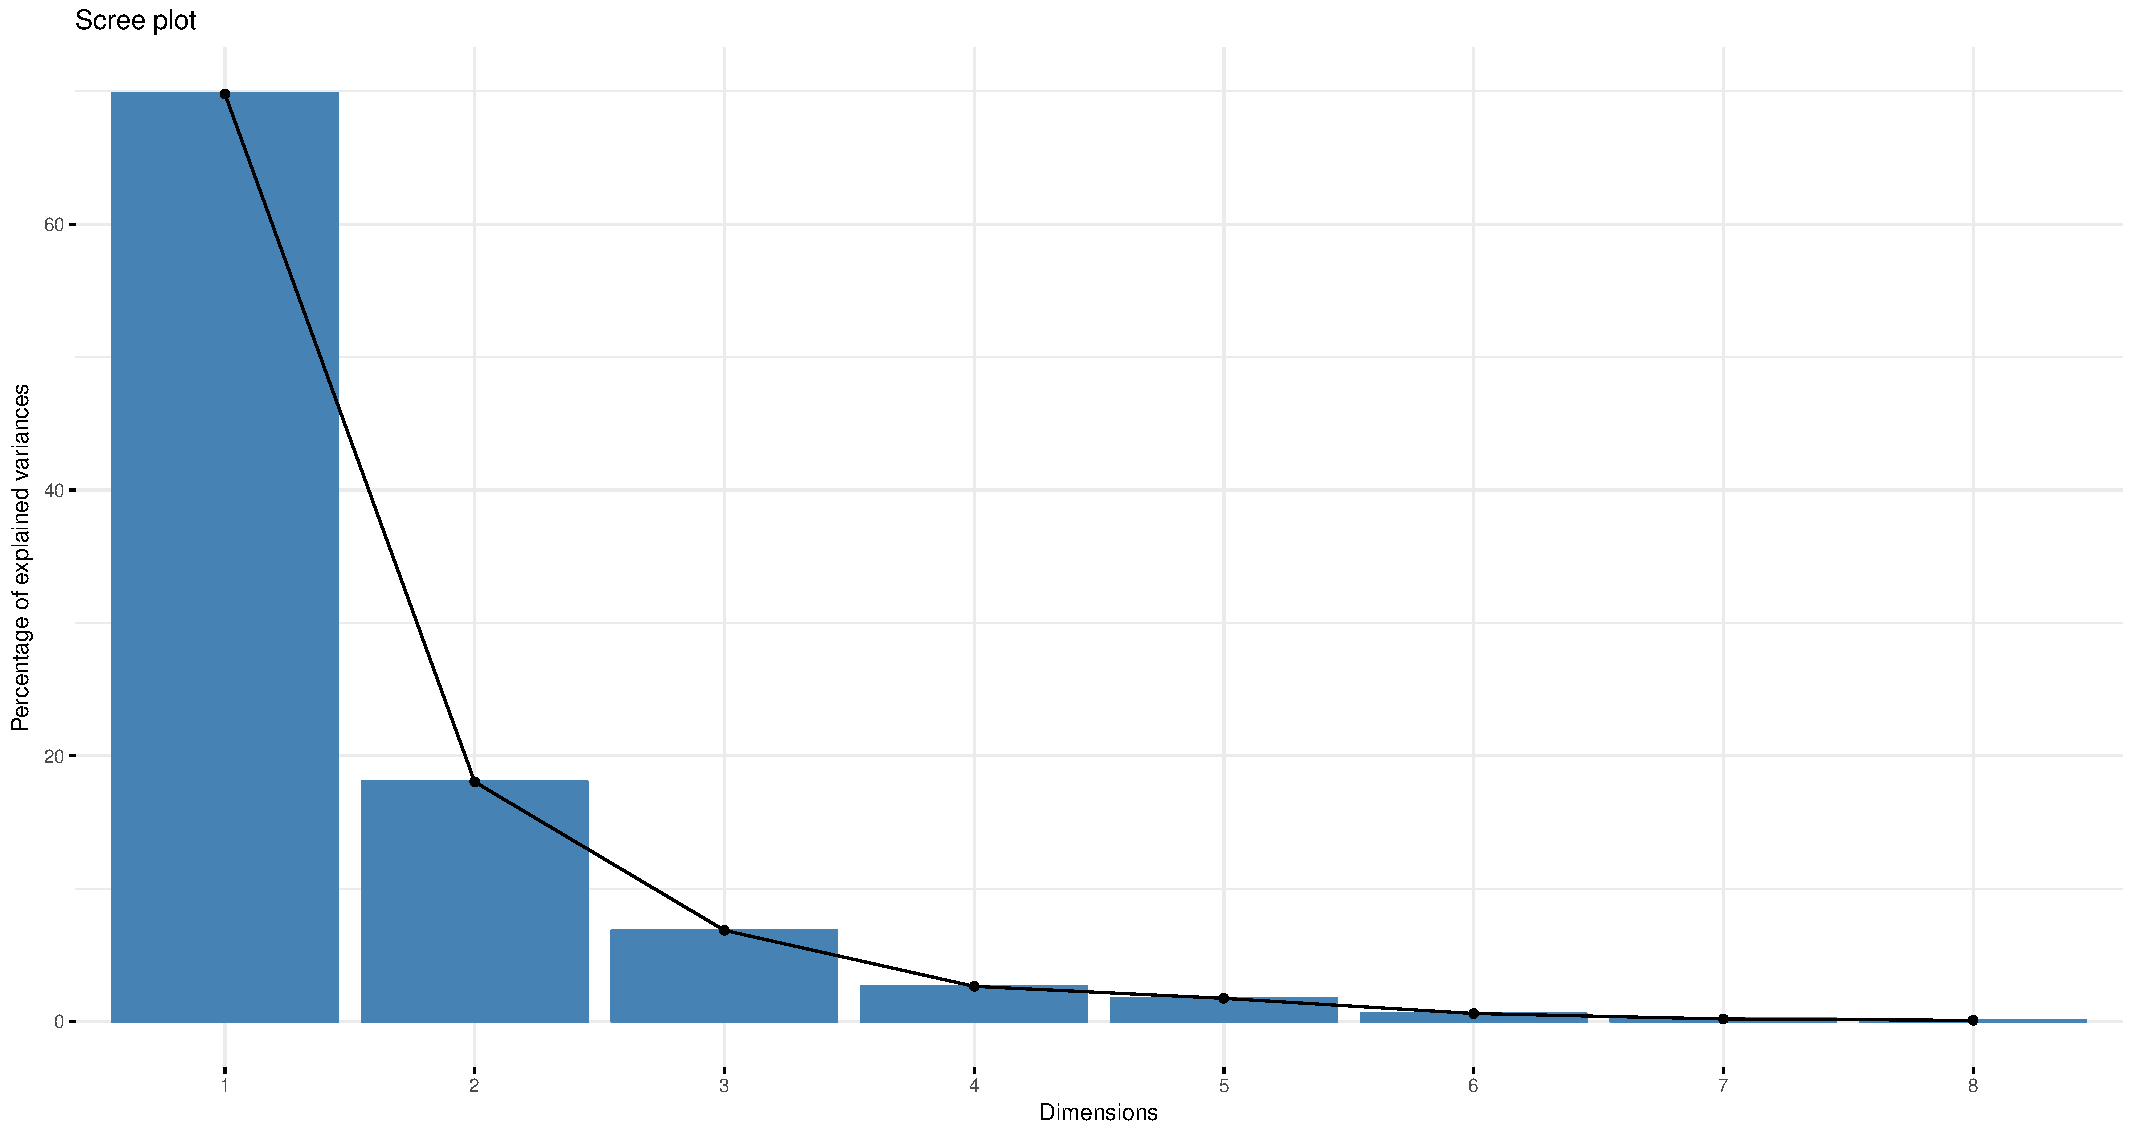
\includegraphics[scale=0.34]{imagenes/I.pdf}
\end{figure}
\end{frame}

\begin{frame}
\frametitle{Resultados para los individuos}
\begin{itemize}
\item Coordenadas
\end{itemize}
\begin{center}
\begin{tabular}{|c|c|c|}
\hline
 & Dim.1  &     Dim.2 \\
\hline
1 & -1.3143364&  0.66717540 \\
2 & -0.3841853&  0.79937921\\
3 & -1.0565914&  0.62799661\\
4 &  2.9064639& -0.12345710\\
5 &  1.4632792&  0.92058312\\
6 &  0.4665257&  0.06981062\\
7 & -0.2300072& -0.89133817\\
8 & -0.5225866& -1.13568796\\
9 &  0.1370254& -0.90435088\\
10& -1.3937676& -0.67628794\\
11& -1.7680431&  0.54456430\\
12&  1.6962234&  0.10161280\\
\hline
\end{tabular}
\end{center}
\end{frame}

\begin{frame}
\frametitle{Resultados para los individuos}
\begin{itemize}
\item Nube de individuos
\end{itemize}
\begin{figure}[h]
  \centering
  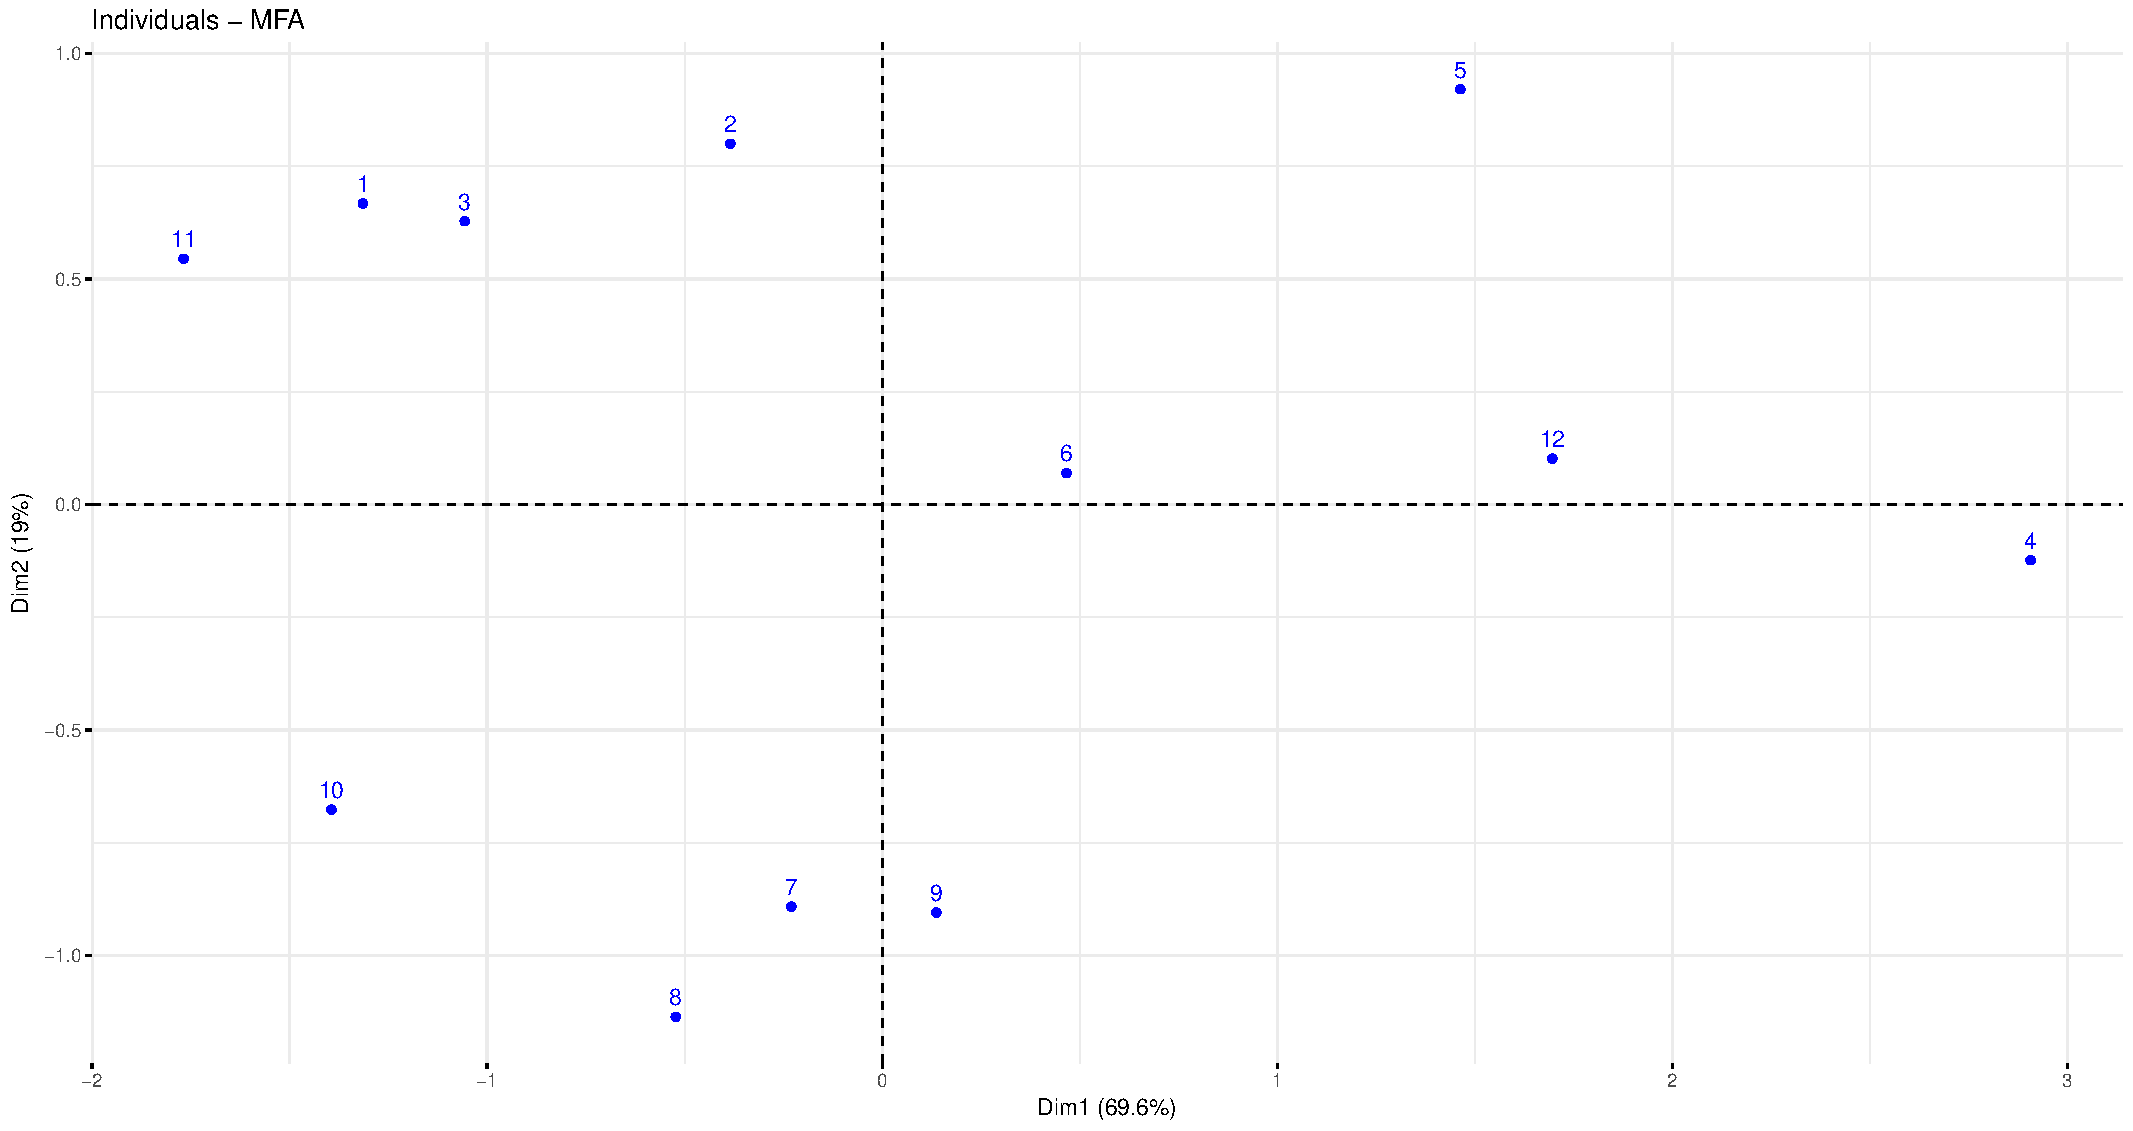
\includegraphics[scale=0.32]{imagenes/nubeind.pdf}
\end{figure}
\end{frame}

\begin{frame}
\frametitle{Resultados para los individuos}
\begin{itemize}
\item Contribuciones
\end{itemize}
\begin{center}
\begin{tabular}{|c|c|c|}
\hline
 & Dim.1  &     Dim.2 \\
\hline
1 &  7.82077792&  7.40334197 \\
2 &  0.66821834& 10.62804681\\
3 &  5.05418322&  6.55937355\\
4 & 38.24430069&  0.25350113\\
5 &  9.69373756& 14.09528211\\
6 &  0.98534439&  0.08105705\\
7 &  0.23950776& 13.21395346\\
8 &  1.23638399& 21.45190194\\
9 &  0.08500387& 13.60259270\\
10 & 8.79463025&  7.60695852\\
11 &14.15215481&  4.93226139\\
12 &13.02575720&  0.17172937\\
\hline
\end{tabular}
\end{center}
\end{frame}

\begin{frame}
\frametitle{Resultados para los individuos}
\begin{itemize}
\item Contribuciones
\end{itemize}
\begin{figure}[h]
  \centering
  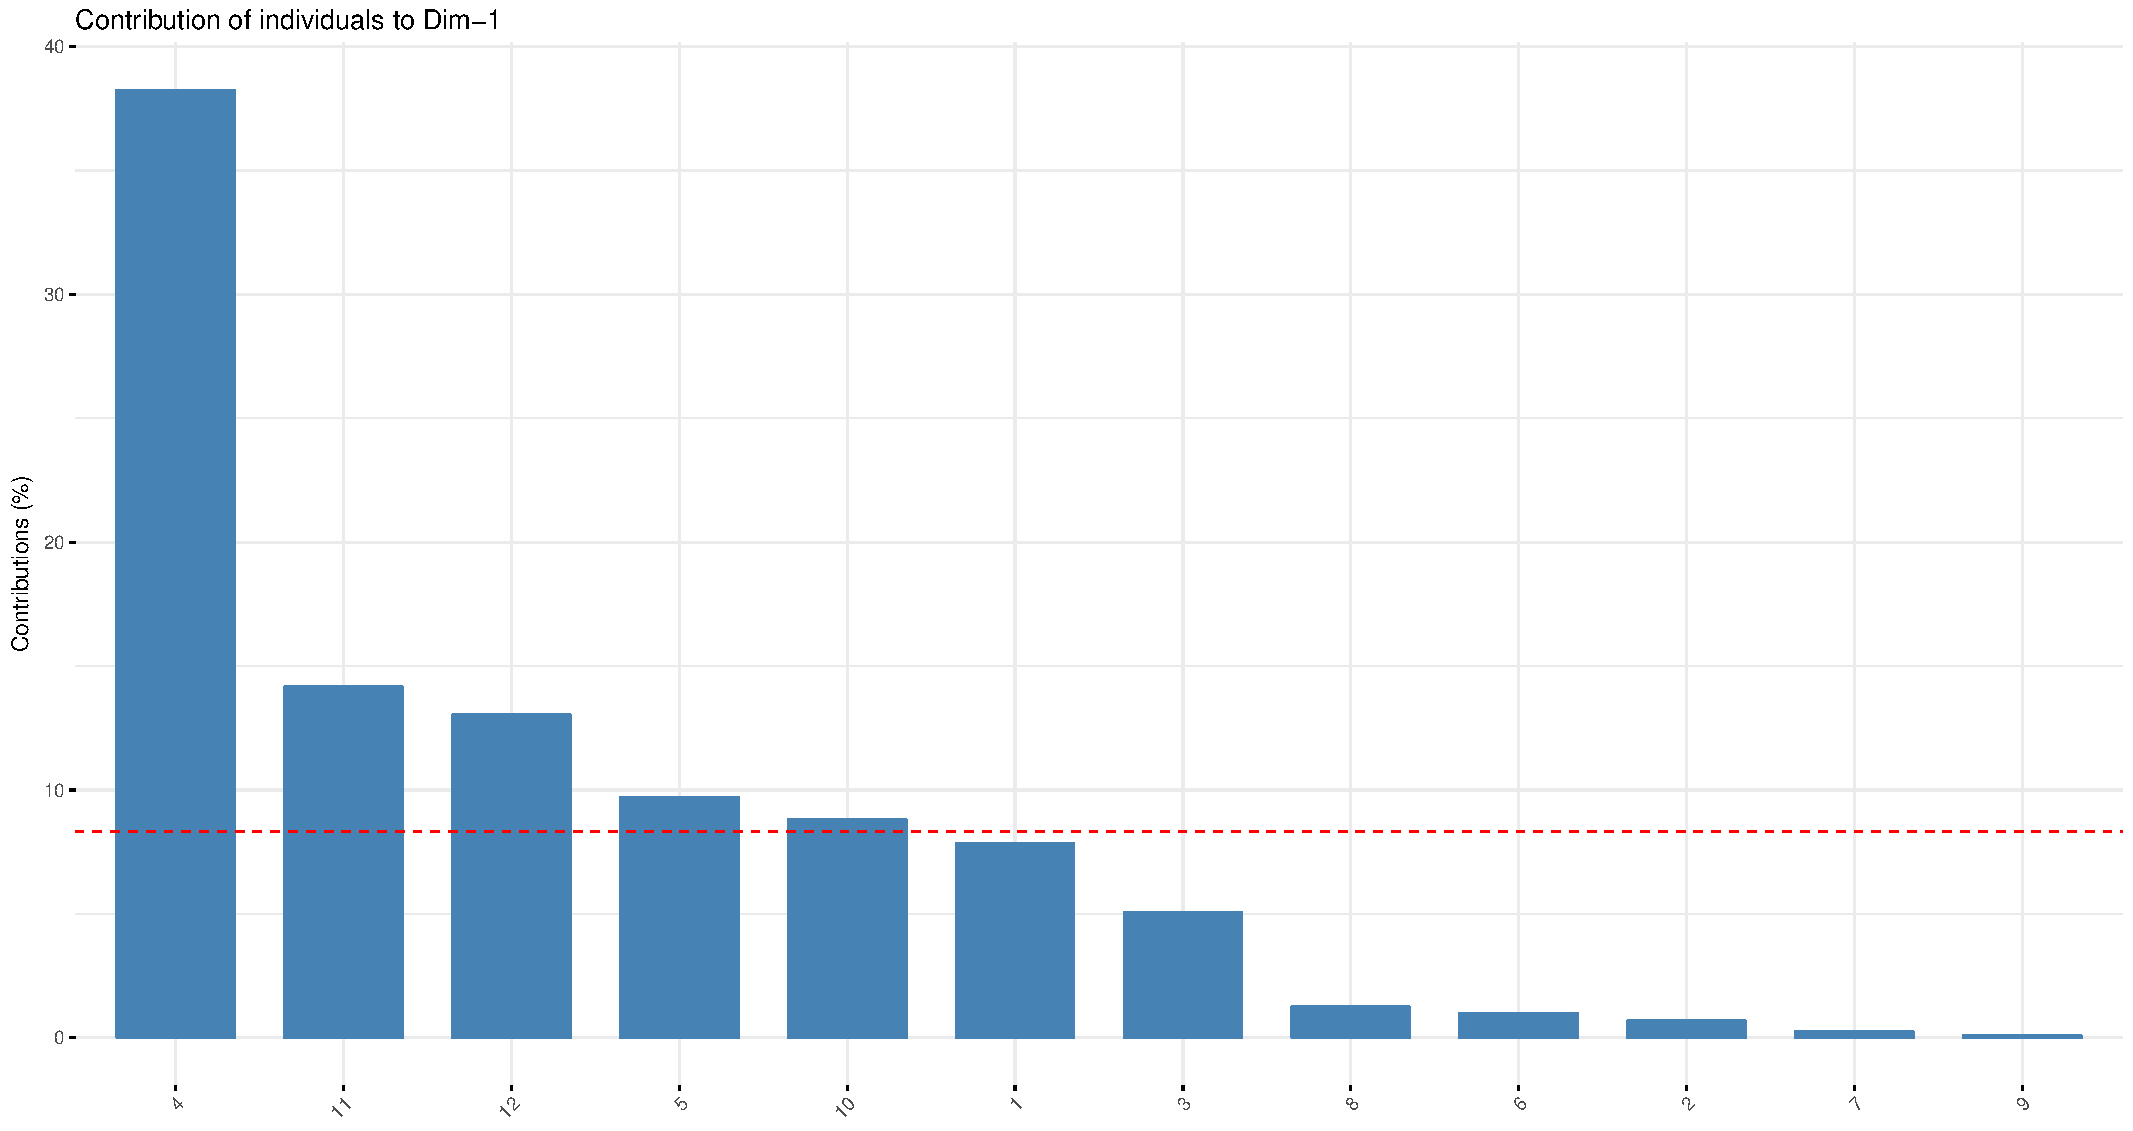
\includegraphics[scale=0.33]{imagenes/CID1.pdf}
\end{figure}
\end{frame}

\begin{frame}
\frametitle{Resultados para los individuos}
\begin{itemize}
\item Contribuciones
\end{itemize}
\begin{figure}[h]
  \centering
  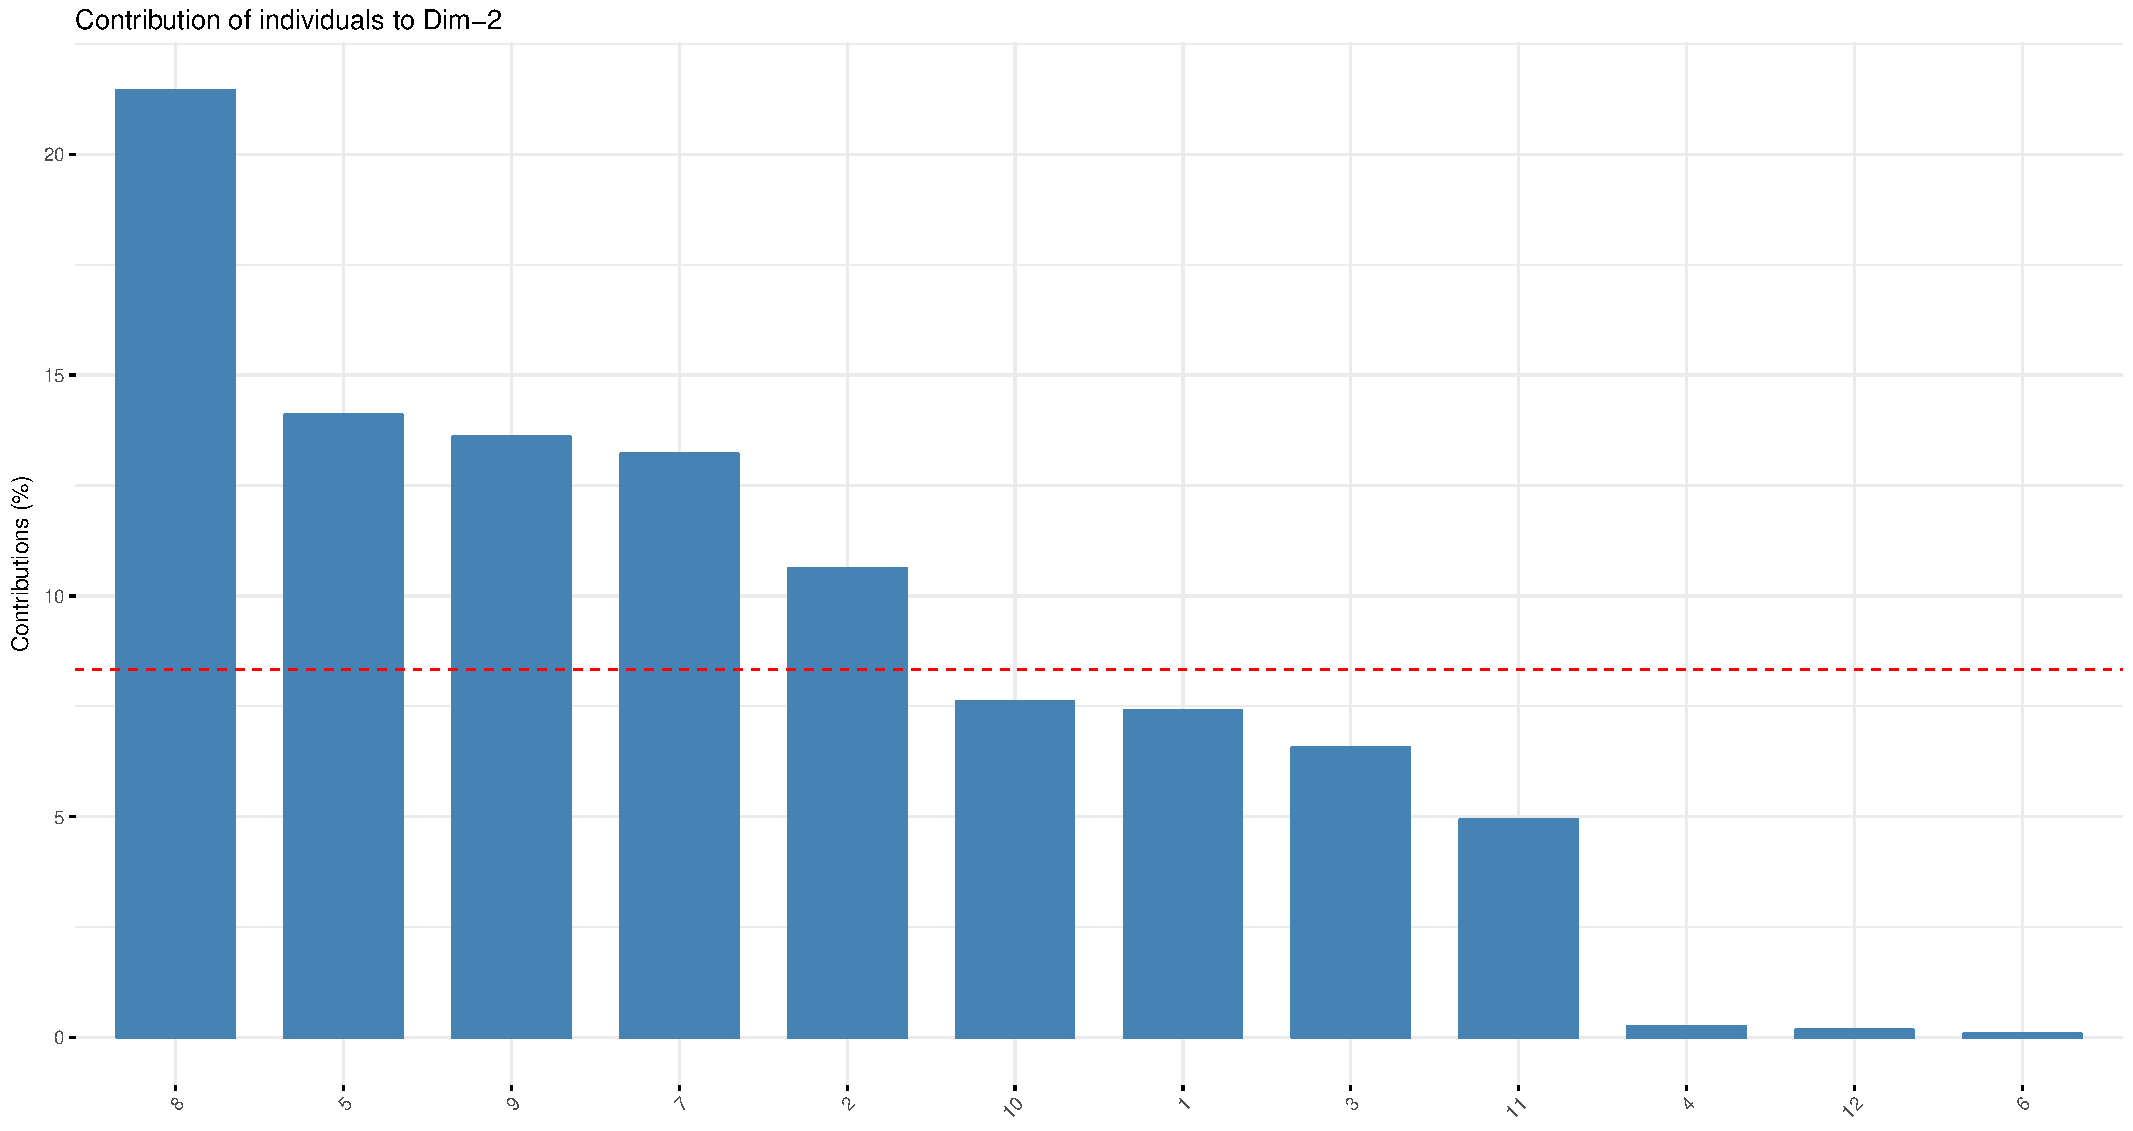
\includegraphics[scale=0.33]{imagenes/CID2.pdf}
\end{figure}
\end{frame}

\begin{frame}
\frametitle{Resultados para los individuos}
\begin{itemize}
\item Cosenos cuadrados
\end{itemize}
\begin{center}
\begin{tabular}{|c|c|c|}
\hline
 & Dim.1  &     Dim.2 \\
\hline
1 & 0.78366123& 0.201927428 \\
2 & 0.10365480& 0.448759438\\
3 & 0.72290537& 0.255377089\\
4 & 0.97704556& 0.001762857\\
5 & 0.65512731& 0.259296895\\
6 & 0.17896249& 0.004007318\\
7 & 0.04884725& 0.733571370\\
8 & 0.16466255& 0.777671827\\
9 & 0.01490332& 0.649165033\\
10& 0.73853508& 0.173881625\\
11& 0.88421345& 0.083882184\\
12& 0.88317768& 0.003169413\\
\hline
\end{tabular}
\end{center}
\end{frame}

\begin{frame}
\frametitle{Resultados para los individuos}
\begin{itemize}
\item Cosenos cuadrados
\end{itemize}
\begin{figure}[h]
  \centering
  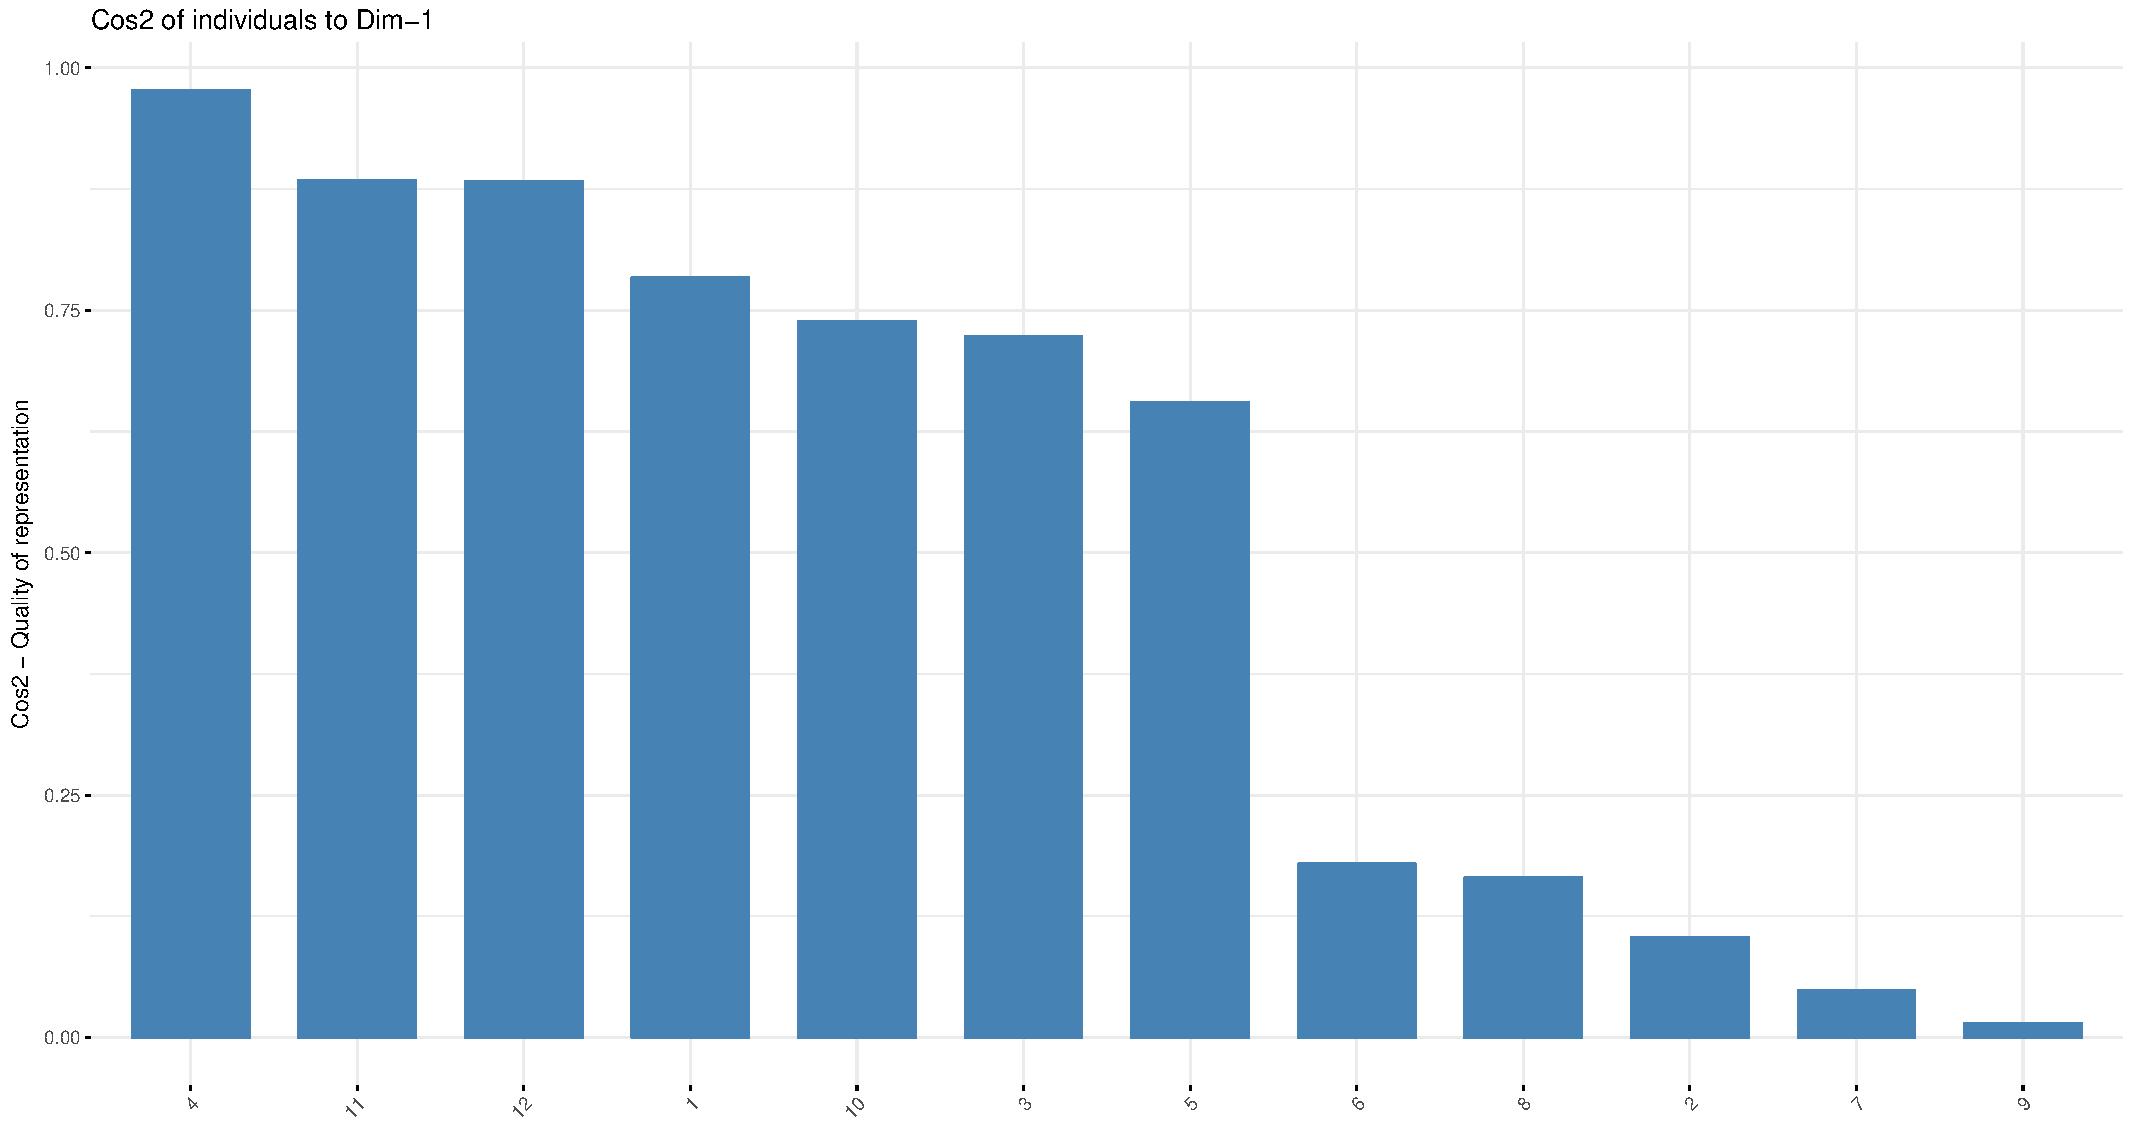
\includegraphics[scale=0.33]{imagenes/C2ID1.pdf}
\end{figure}
\end{frame}

\begin{frame}
\frametitle{Resultados para los individuos}
\begin{itemize}
\item Cosenos cuadrados
\end{itemize}
\begin{figure}[h]
  \centering
  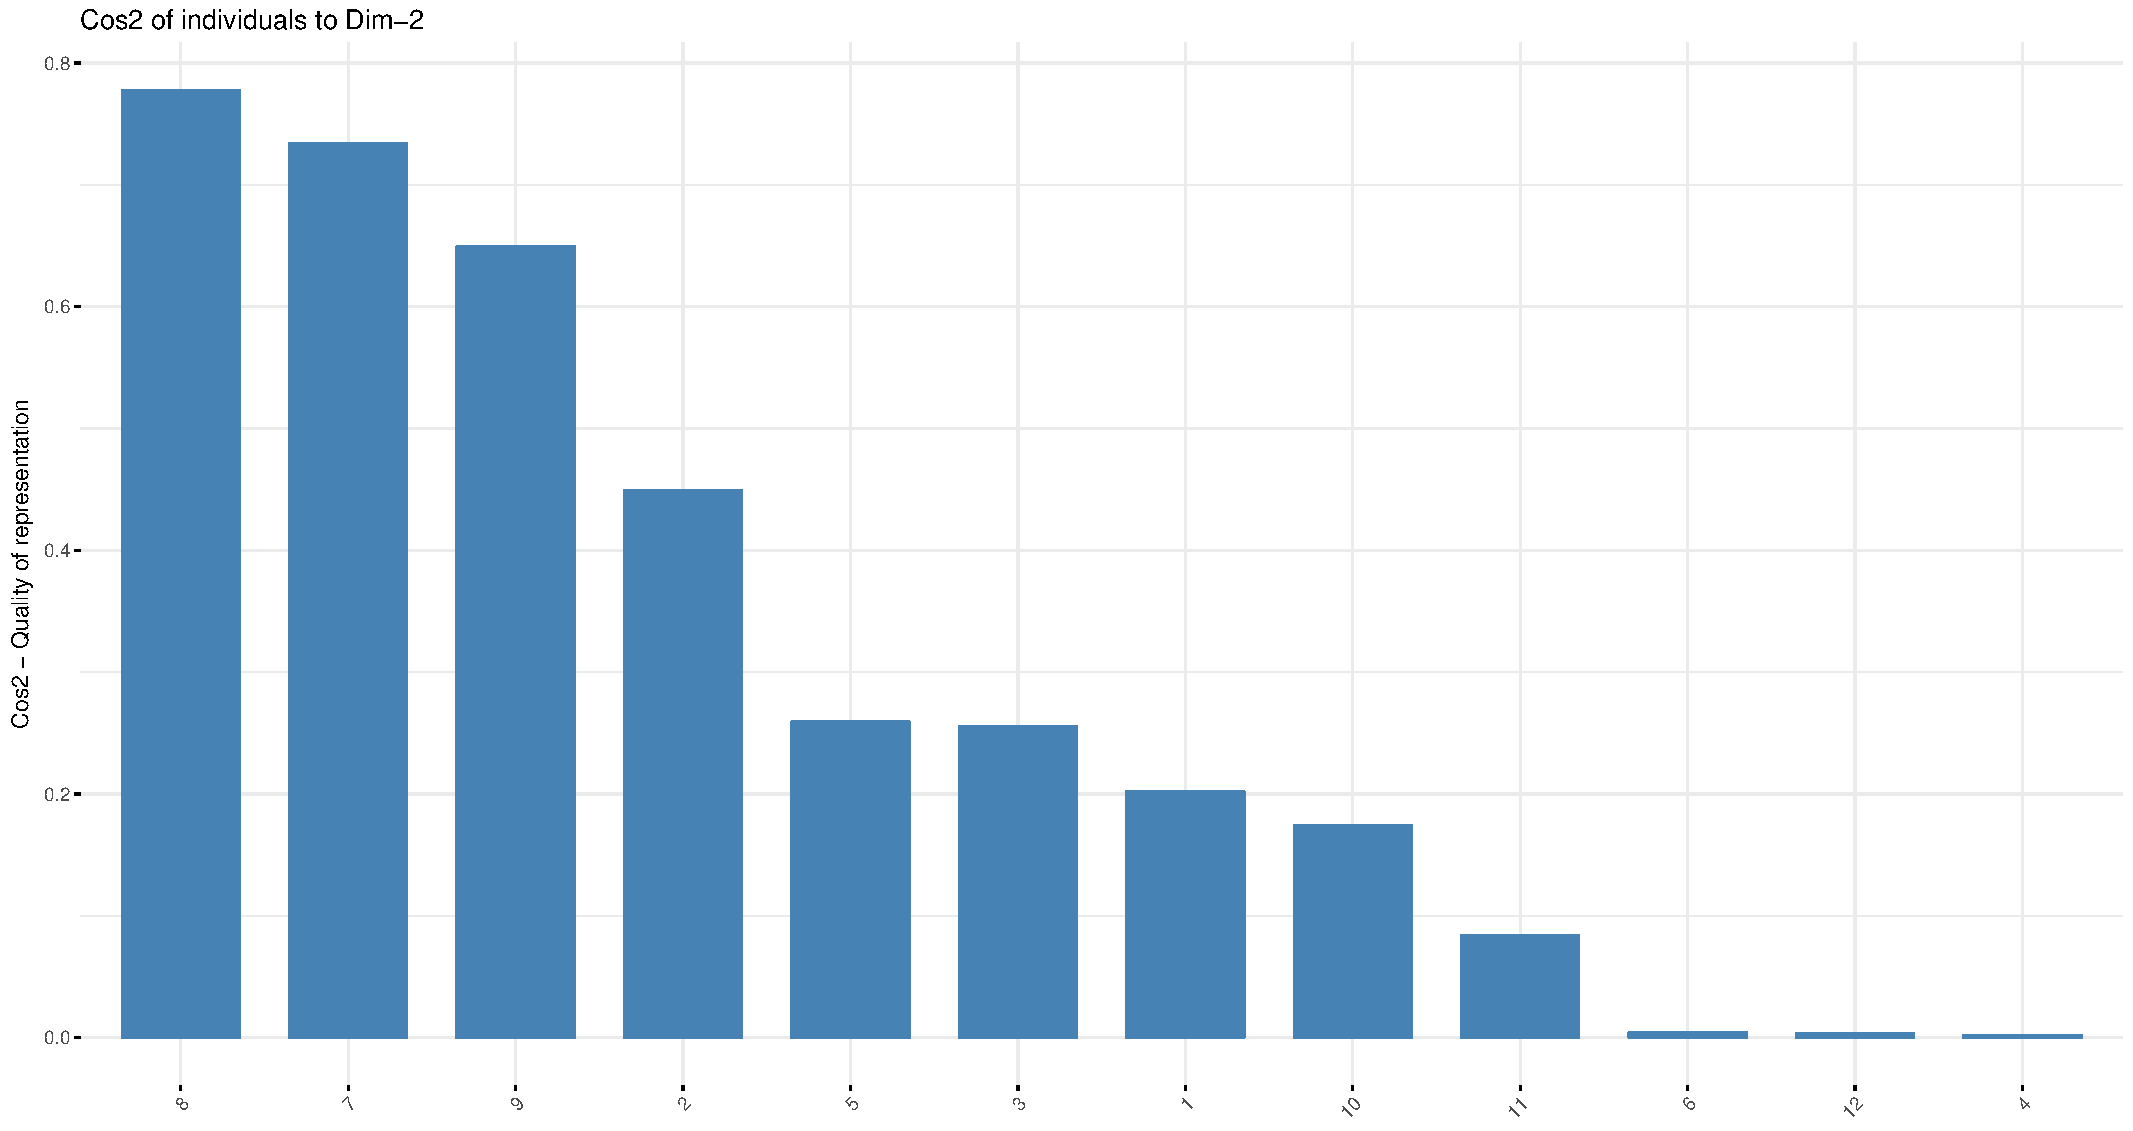
\includegraphics[scale=0.33]{imagenes/C2ID2.pdf}
\end{figure}
\end{frame}

\begin{frame}
\frametitle{Resultados para las variables}
\begin{itemize}
\item Coordenadas
\end{itemize}
\begin{center}
\begin{tabular}{|c|c|c|}
\hline
 & Dim.1  &     Dim.2 \\
\hline
Color.intensity  &  0.8542630 & 0.28809072 \\
Odor.intensity   & 0.6141905 & 0.71649921\\
Attack.intensity & 0.9502405 &-0.23400493\\
Sweet           & -0.8979722 &-0.07642941\\
Acid            &  0.9039337 &-0.31789113\\
Bitter          &  0.9697080 & 0.17204423\\
Pulp            & -0.6398293 & 0.70466313\\
Typicity        & -0.8053443 & 0.40789439\\
\hline
\end{tabular}
\end{center}
\end{frame}

\begin{frame}
\frametitle{Resultados para las variables}
\begin{itemize}
\item Nube de variables
\end{itemize}
\begin{figure}[h]
  \centering
  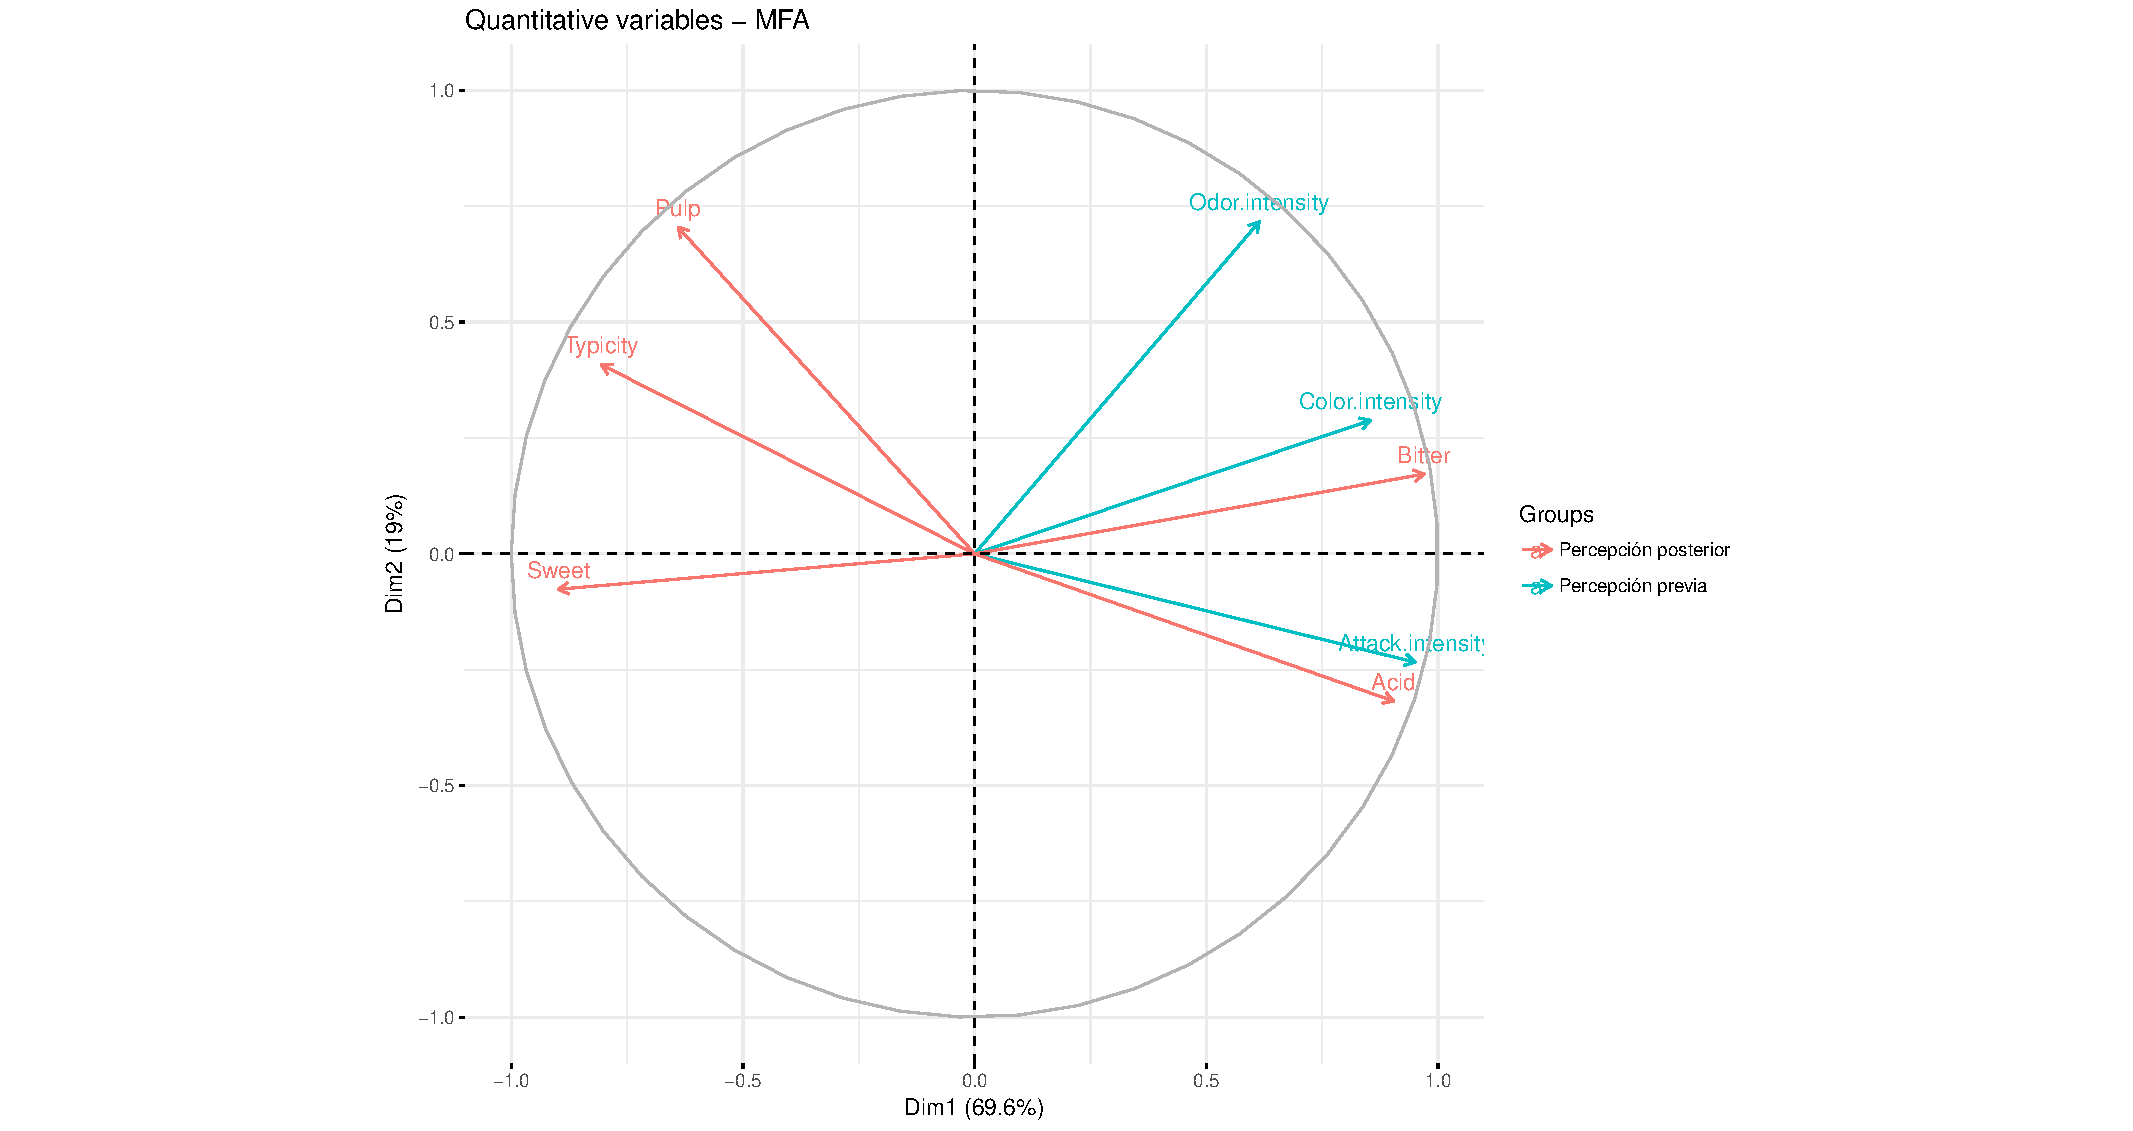
\includegraphics[scale=0.32]{imagenes/nubevar.pdf}
\end{figure}
\end{frame}

\begin{frame}
\frametitle{Resultados para las variables}
\begin{itemize}
\item Contribuciones
\end{itemize}
\begin{center}
\begin{tabular}{|c|c|c|}
\hline
 & Dim.1  &     Dim.2 \\
\hline
Color.intensity &  18.104829&  7.5645086\\
Odor.intensity  &  9.358741& 46.7900601\\
Attack.intensity& 22.401565&  4.9908234\\
Sweet           & 11.162149&  0.2970666\\
Acid            & 11.310847&  5.1391316\\
Bitter          & 13.016792&  1.5052657\\
Pulp            &  5.666961& 25.2520138\\
Typicity        &  8.978116&  8.4611302\\
\hline
\end{tabular}
\end{center}
\end{frame}

\begin{frame}
\frametitle{Resultados para las variables}
\begin{itemize}
\item Contribuciones
\end{itemize}
\begin{figure}[h]
  \centering
  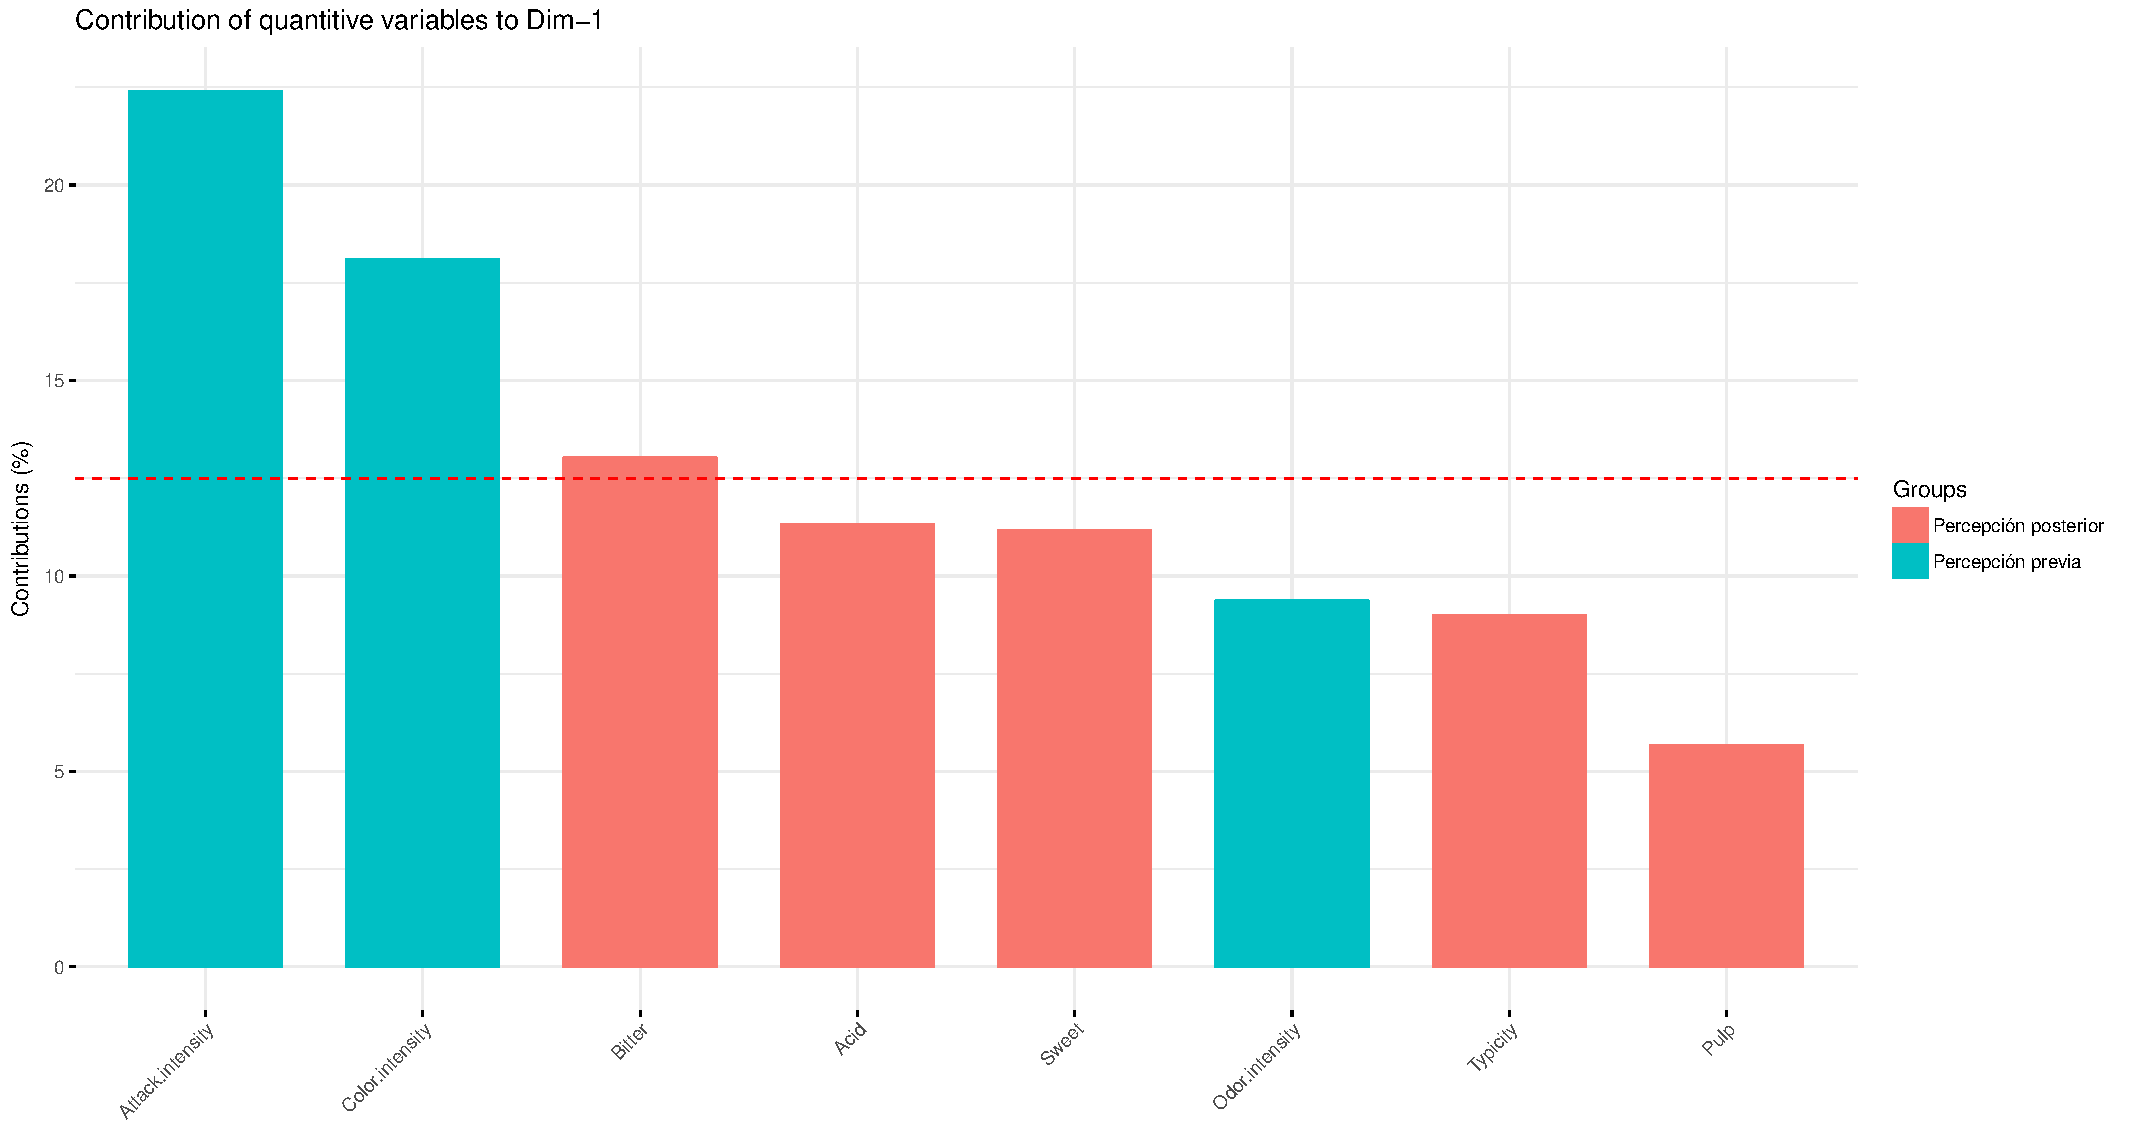
\includegraphics[scale=0.33]{imagenes/CVD1.pdf}
\end{figure}
\end{frame}

\begin{frame}
\frametitle{Resultados para las variables}
\begin{itemize}
\item Contribuciones
\end{itemize}
\begin{figure}[h]
  \centering
  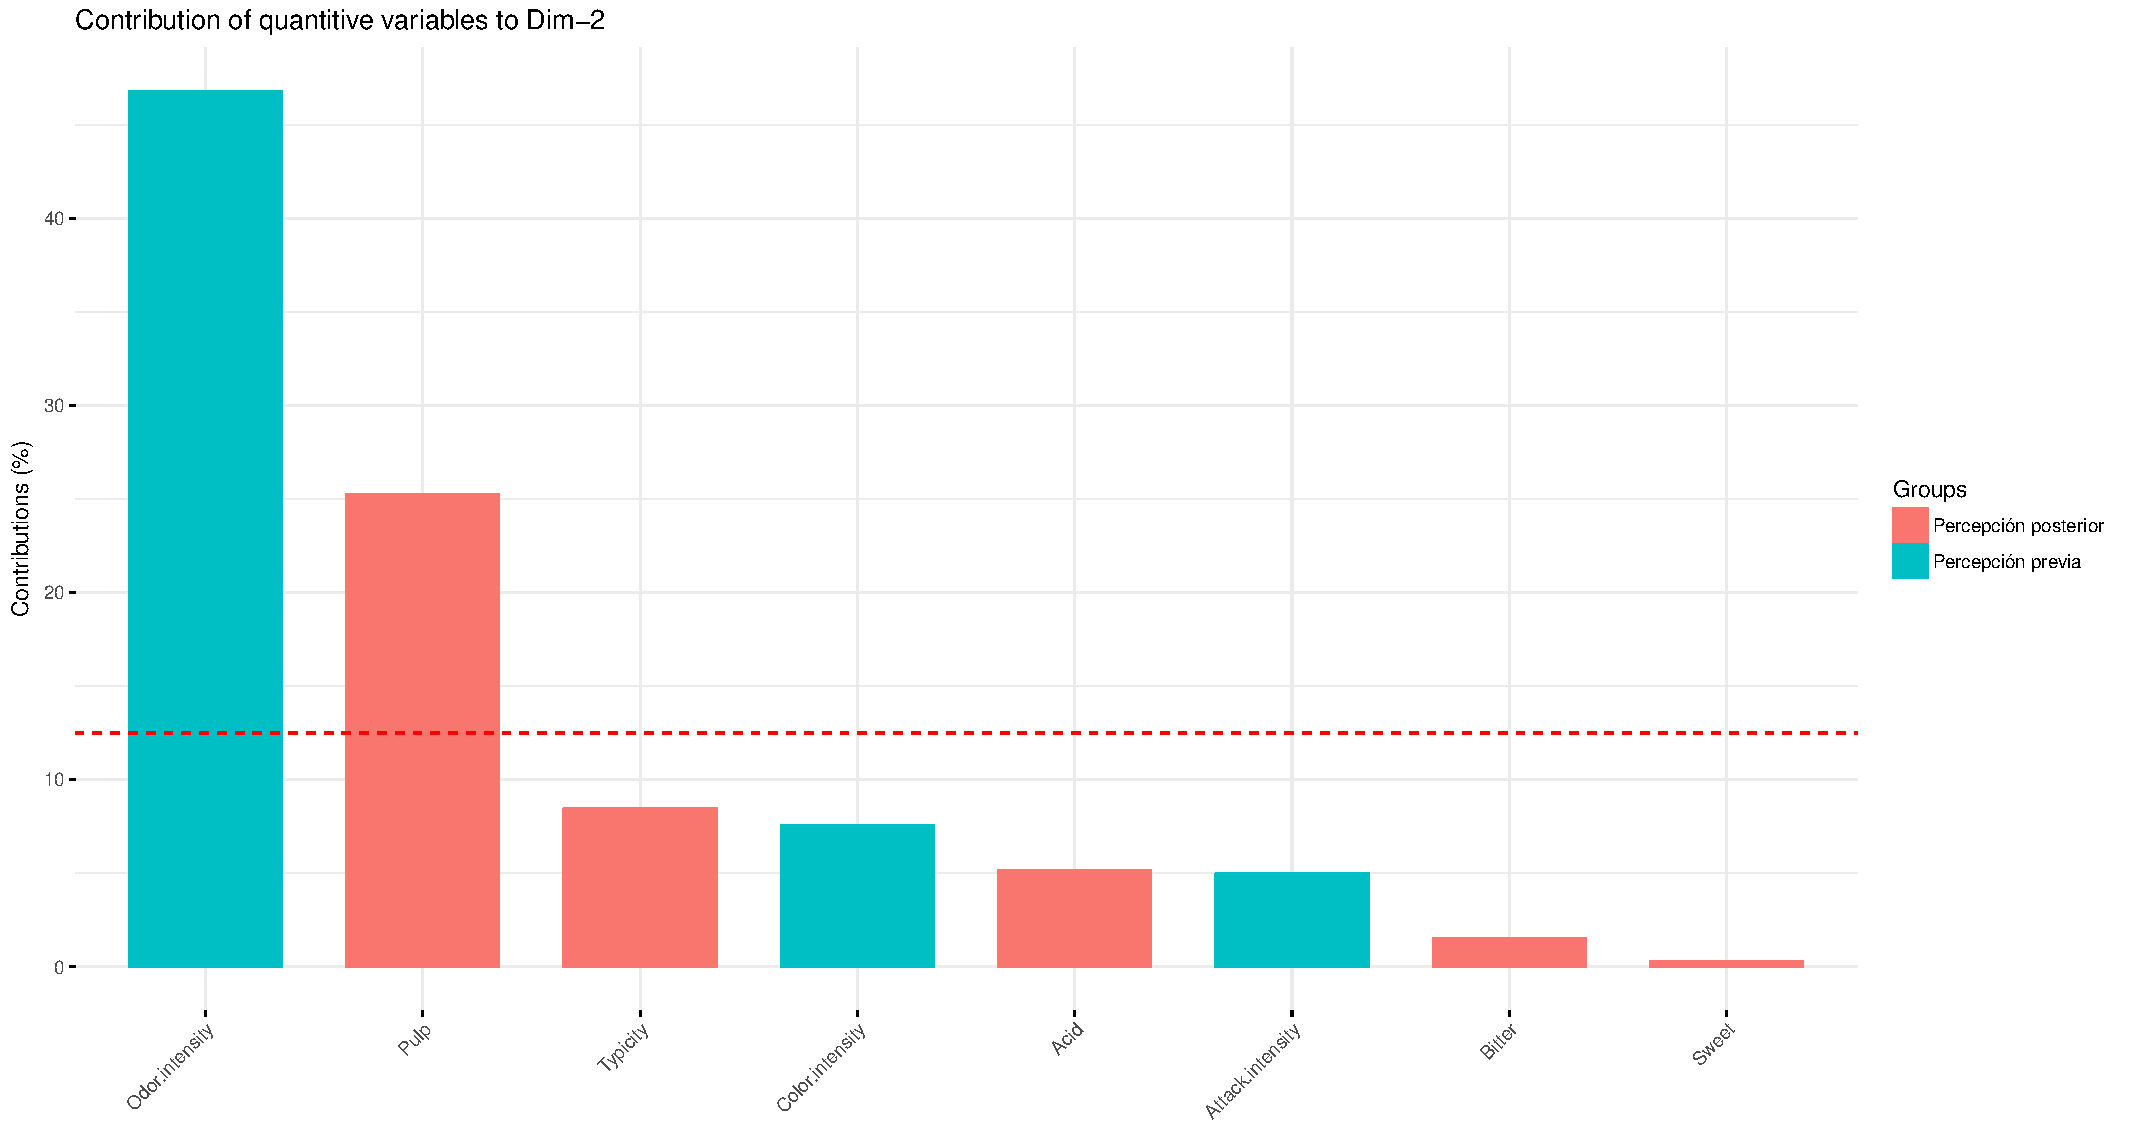
\includegraphics[scale=0.33]{imagenes/CVD2.pdf}
\end{figure}
\end{frame}

\begin{frame}
\frametitle{Resultados para las variables}
\begin{itemize}
\item Cosenos cuadrados
\end{itemize}
\begin{center}
\begin{tabular}{|c|c|c|}
\hline
 & Dim.1  &     Dim.2 \\
\hline
Color.intensity & 0.7297652 &0.082996266 \\
Odor.intensity  & 0.3772299 &0.513371117\\
Attack.intensity& 0.9029570 &0.054758309\\
Sweet           & 0.8063541 &0.005841454\\
Acid            & 0.8170961 &0.101054769\\
Bitter          & 0.9403336 &0.029599218\\
Pulp            & 0.4093815 &0.496550127\\
Typicity        & 0.6485794 &0.166377831\\
\hline
\end{tabular}
\end{center}
\end{frame}

\begin{frame}
\frametitle{Resultados para las variables}
\begin{itemize}
\item Cosenos cuadrados
\end{itemize}
\begin{figure}[h]
  \centering
  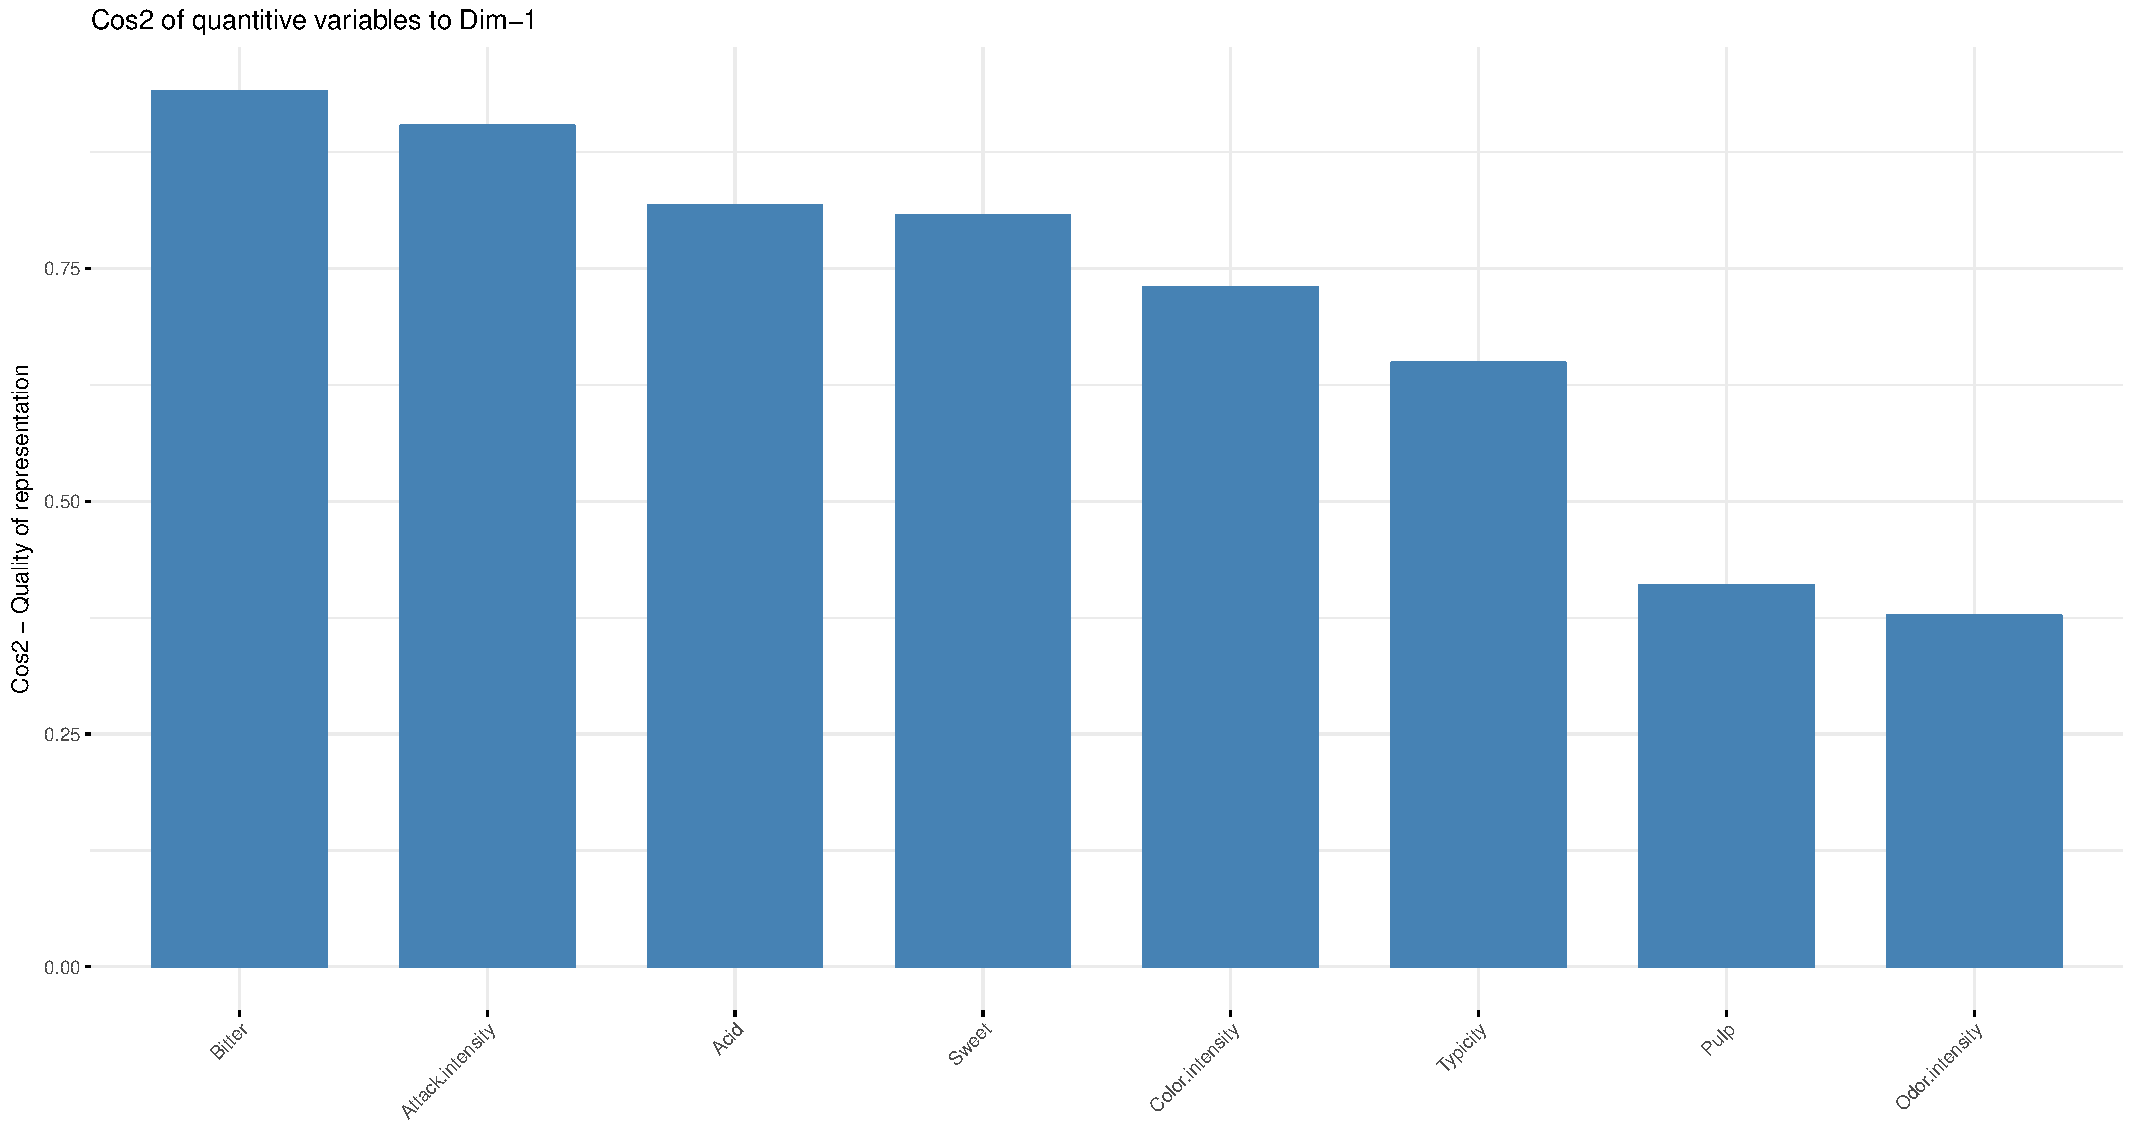
\includegraphics[scale=0.33]{imagenes/C2VD1.pdf}
\end{figure}
\end{frame}

\begin{frame}
\frametitle{Resultados para las variables}
\begin{itemize}
\item Cosenos cuadrados
\end{itemize}
\begin{figure}[h]
  \centering
  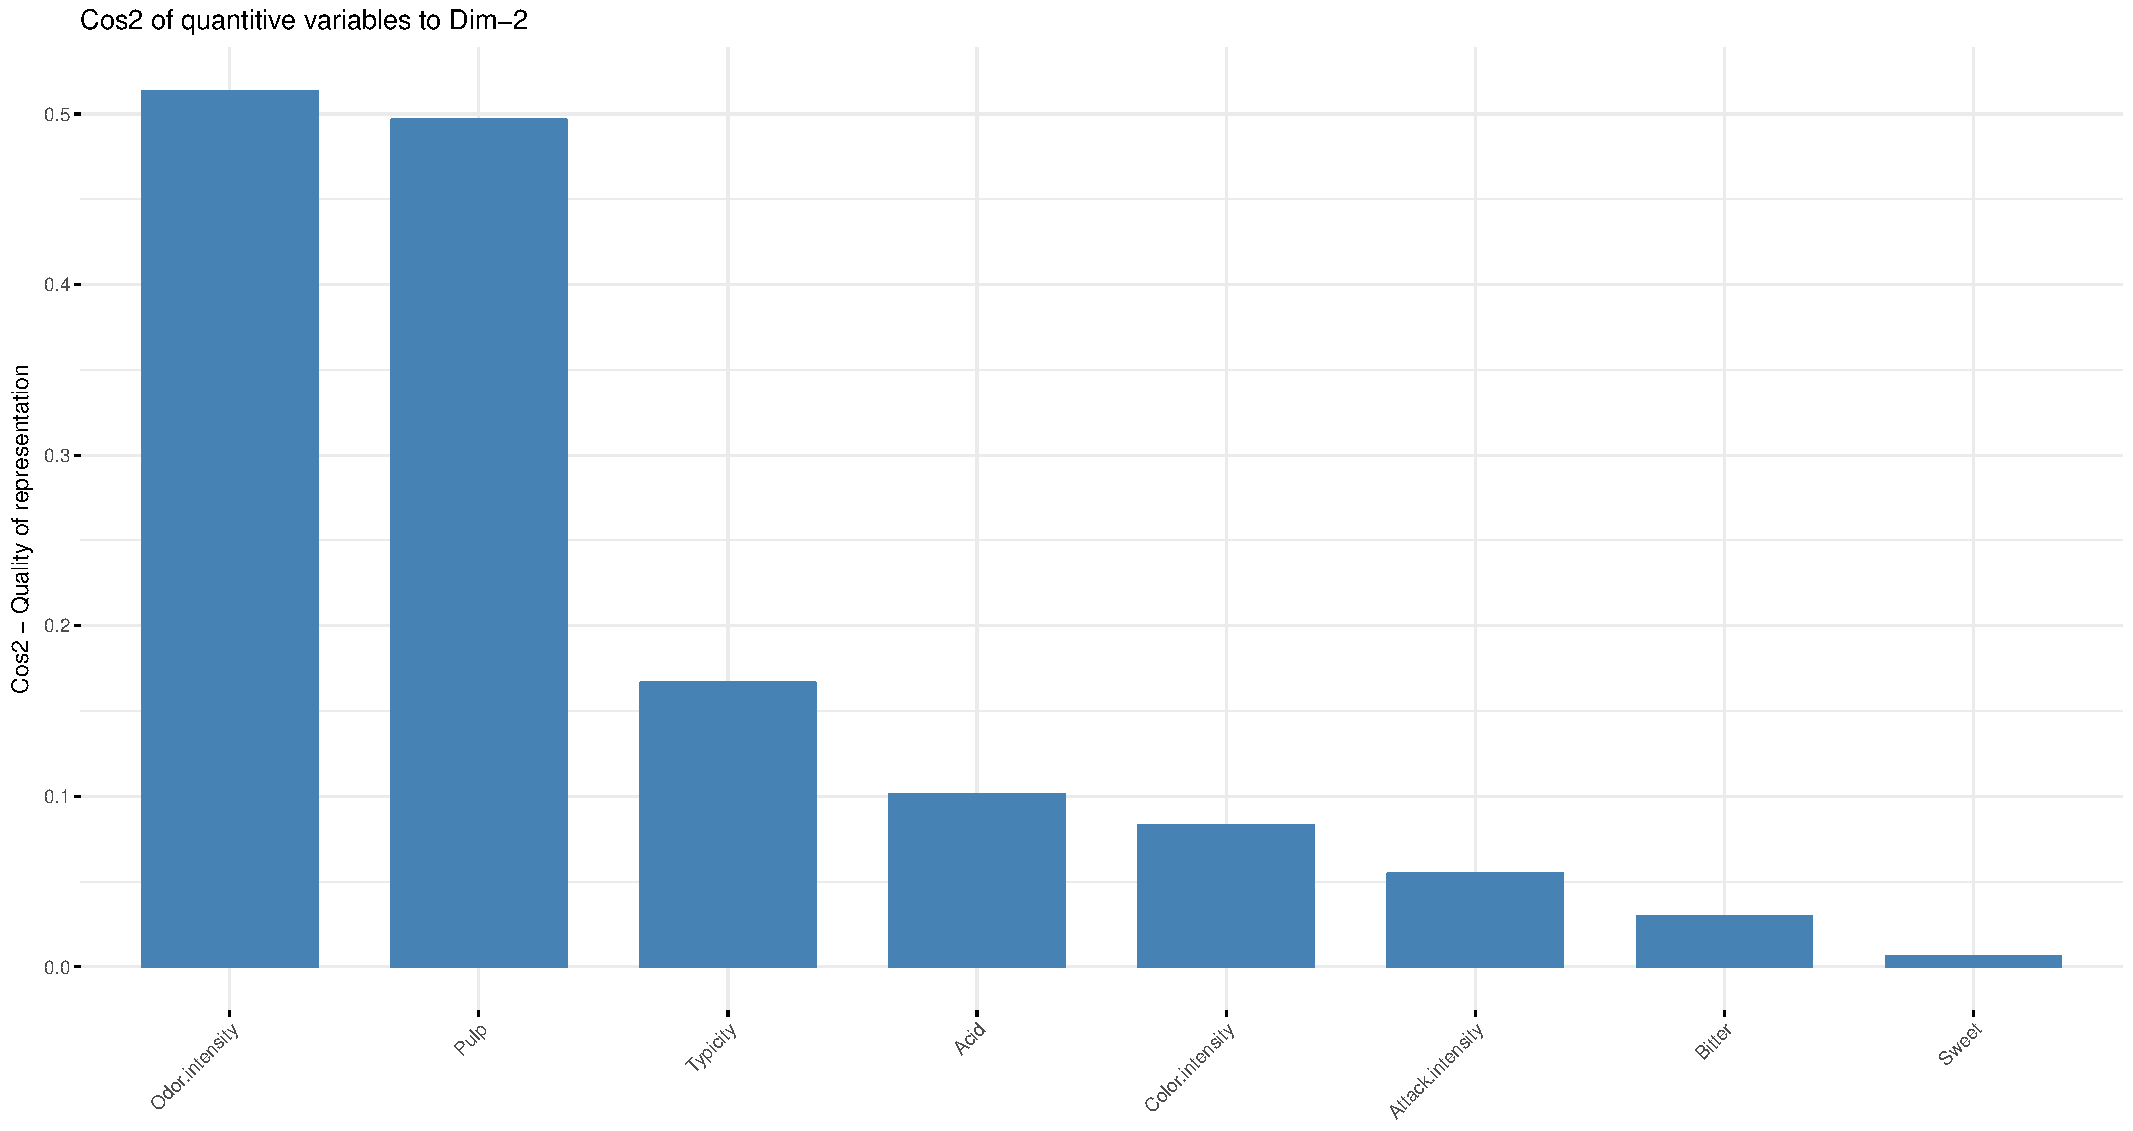
\includegraphics[scale=0.33]{imagenes/C2VD2.pdf}
\end{figure}
\end{frame}


\begin{frame}
\frametitle{Representación simultánea}
\begin{figure}[h]
  \centering
  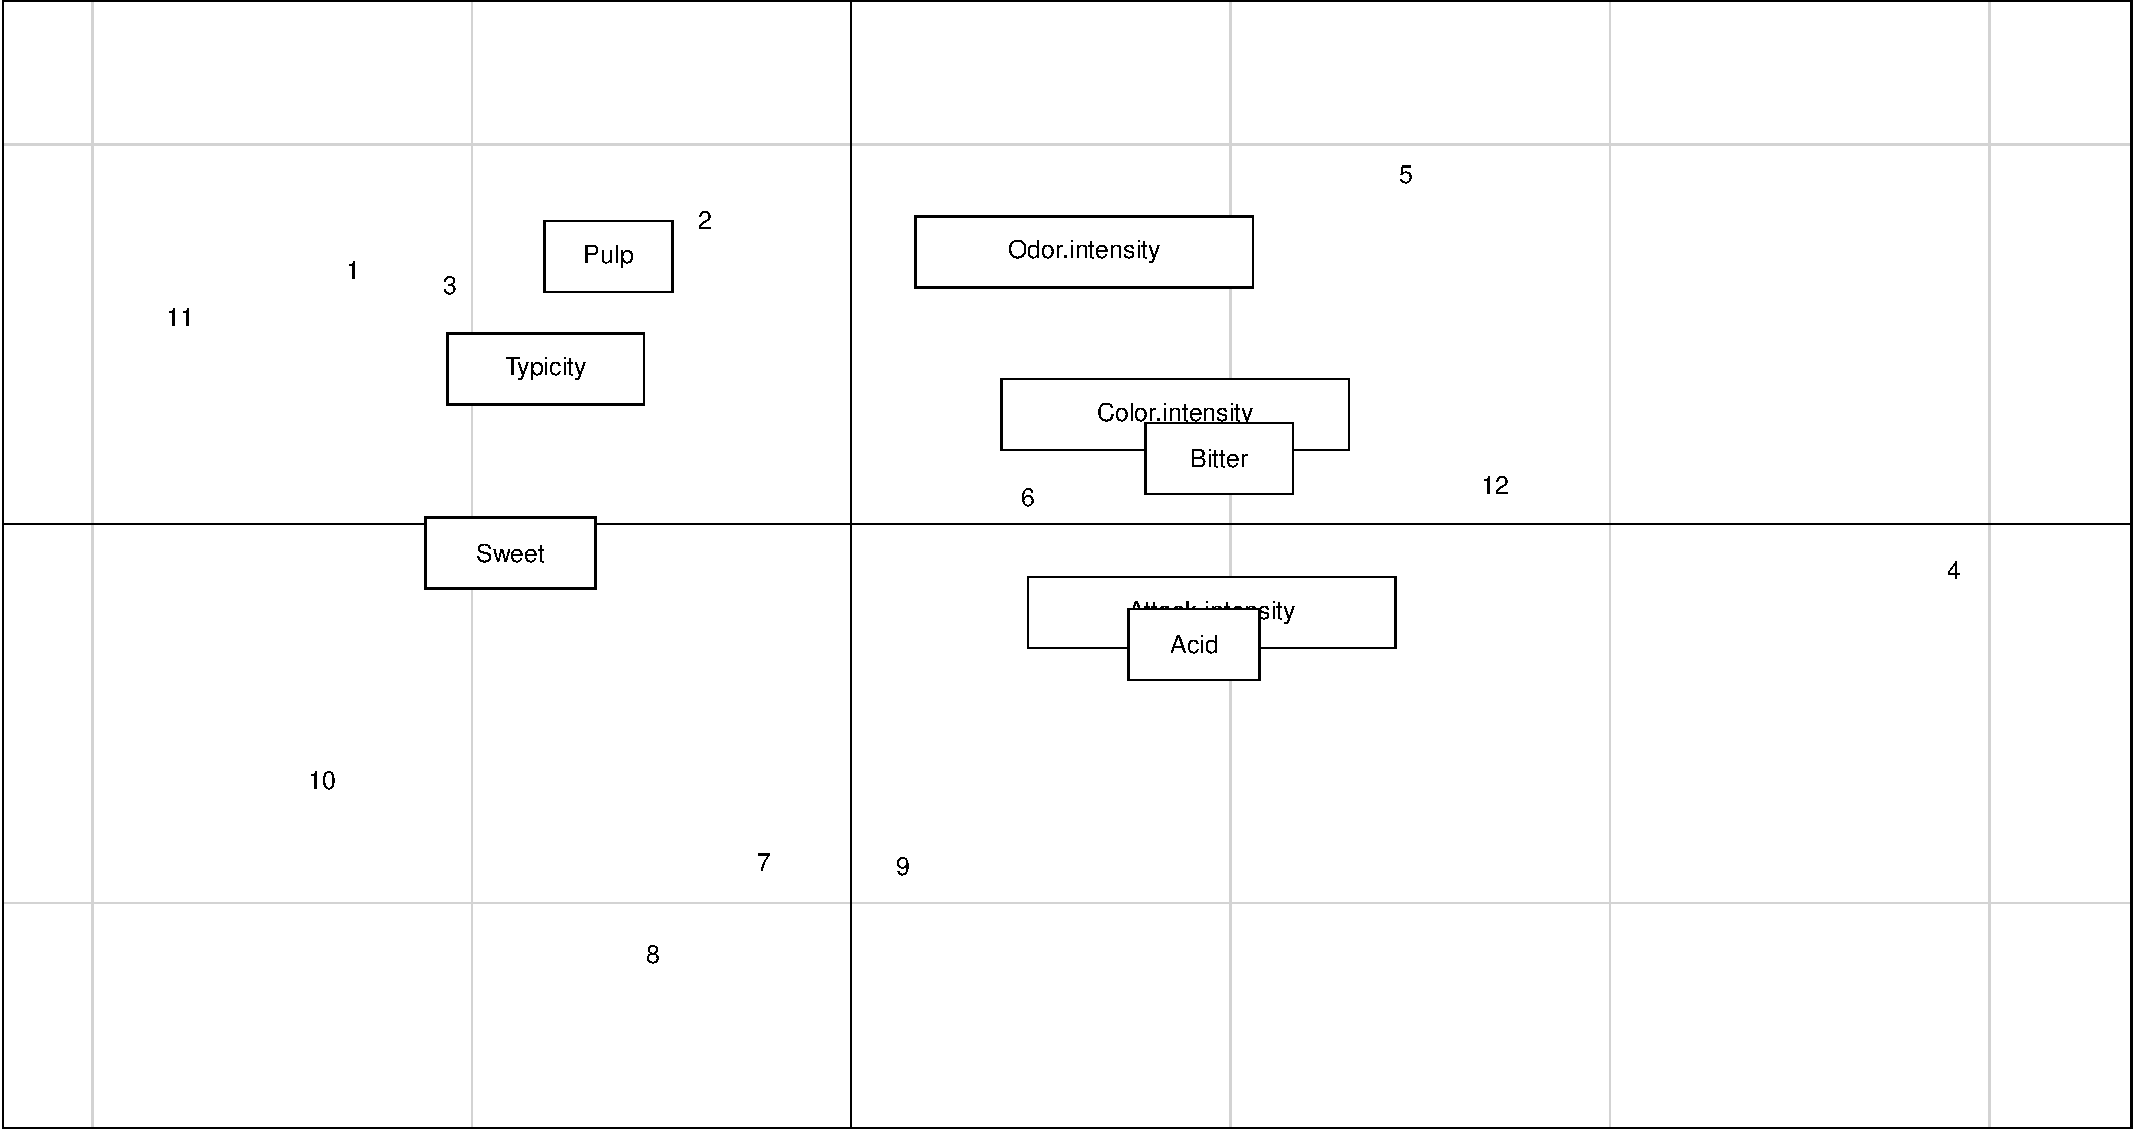
\includegraphics[scale=0.34]{imagenes/RSIM.pdf}
\end{figure}
\end{frame}

\begin{frame}
\frametitle{Nube de los grupos}
\begin{figure}[h]
  \centering
  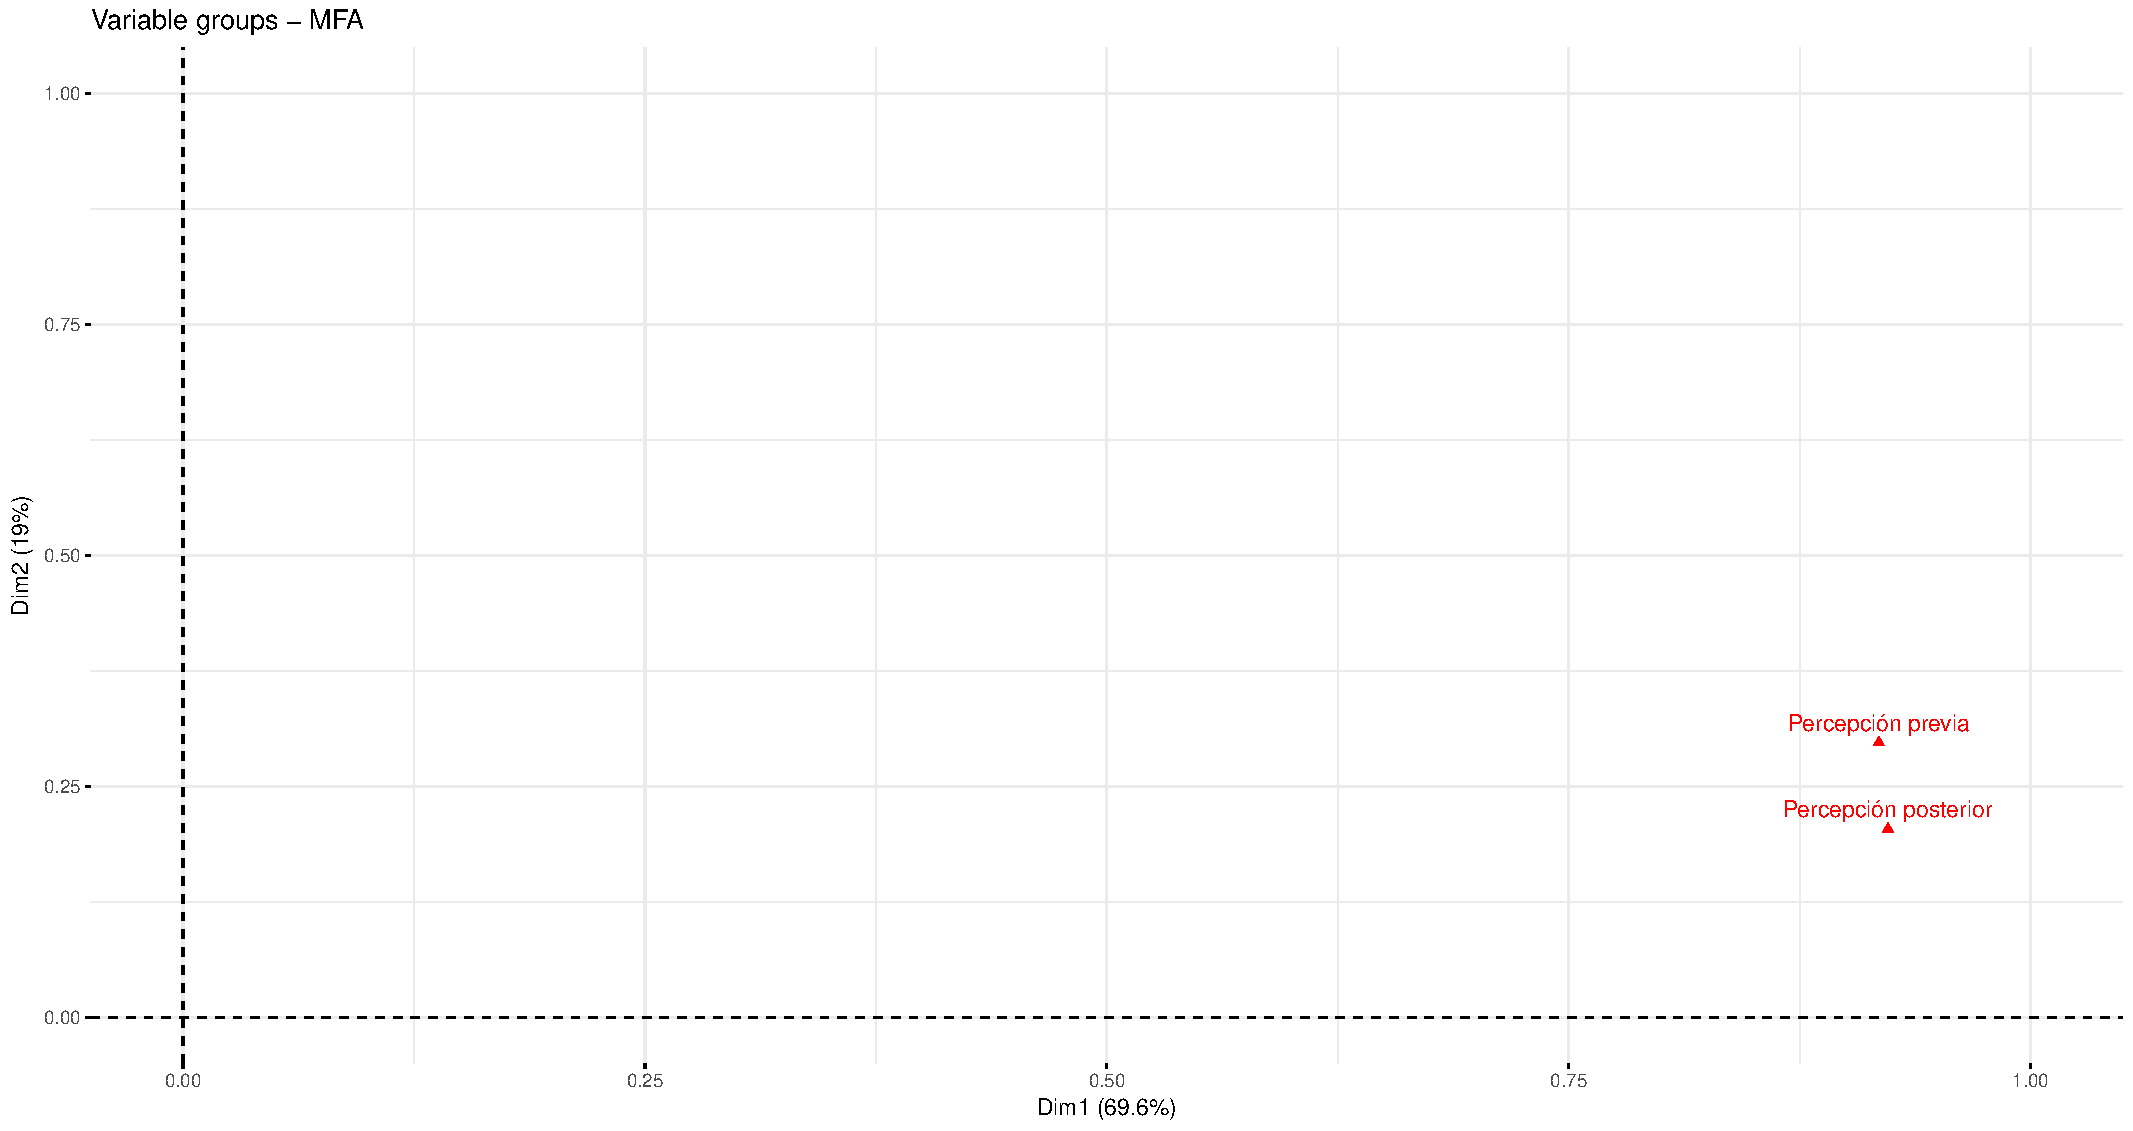
\includegraphics[scale=0.34]{imagenes/nubegru.pdf}
\end{figure}
\end{frame}

\begin{frame}
\frametitle{Coeficiente Lg}
\begin{itemize}
\justifying
\item Coeficiente Lg: Es un indicador del grado de similitud o deformación con respecto a un foco (homotecia) entre los conjuntos
de indicadores, y cuando se calcula para un solo conjunto de ellos. Esto se conoce como indicador de la dimensionalidad de la nube, que es igual al número de direcciones ortogonales de inercia no cero, es decir, el número de valores propios no cero. Esta cantidad es 0 cuando todas las variables de un grupo son ortogonales a todas las variables del otro grupo. Es mas alto en cuanto cada una de las variables de un grupo este más relacionada con el conjunto de variables del otro grupo.
~\\Se define por:
$$Lg=\frac{Traza(S'T)}{\alpha_1^2 x \lambda_1^2}$$
\end{itemize}
\end{frame}

\begin{frame}
\frametitle{Coeficiente Lg}
~\\Los coeficientes Lg se pueden observar en la siguiente tabla:
\begin{center}
\resizebox{12cm}{!}{
\begin{tabular}{cccc}
\hline
 &Percepción previa & Percepción posterior &      MFA\\
Percepción previa   &         1.0839432     &       0.7761085 &1.0105158\\
Percepción posterior       &  0.7761085        &    1.0384112 &0.9857795\\
MFA                       &   1.0105158         &   0.9857795 &1.0845333\\
\hline 
\end{tabular}
} 
\end{center}
~\\El valor del coeficiente $Lg_{(P.Previa)}=1.0839$ para la percepción previa indica que es de dimensionalidad uno, es decir, que puede sintetizarse en un solo factor; $Lg_{(P.Posterior)}=1.0384$ indica que la percepción posterior también tiene una dimensión o factor que lo caracteriza. El coeficiente Lg cruzado $Lg_{(P.Prev,P.Post)}=0.7761$ indica que estos dos grupos comparten un factor; y finalmente, el coeficiente $Lg_{(MFA)}=1.0845$ indica que éste se puede sintetizar como mínimo en un factor.
\end{frame}

\begin{frame}
\frametitle{Coeficiente Rv de Escoufier}
~\\ Es una generalización multivariada del coeficiente de correlación de Pearson al cuadrado. Este coeficiente mide el vínculo entre dos grupos o dos matrices de variables. Este coeficiente, al igual que el de correlación de Pearson, se encuentra entre 0(todas las variables del primer grupo o matriz, son ortogonales a todas las variables del segundo grupo o matriz) y 1(los dos grupos o matrices son homotéticos)

~\\El coeficiente de RV se define como (Robert y Escoufier, 1976; Schlich, 1996):

$$RV(W_i,Wj)=\frac{T(W_i,W_j)}{\left[T(W_i,W_i)\cdot T(W_j,W_j)\right]^\frac{1}{2}}$$
\end{frame}

\begin{frame}
\justifying
\frametitle{Coeficiente Rv de Escoufier}
~\\Donde $T(W_i,W_j)=\sum\limits_{l,m}w_{l,m}^i w_{l,m}^j$ es un coeficiente de covarianza generalizado entre las matrices $W_i$ y $W_j$, $T(W_i,W_i)=\sum\limits_{l,m}{w_{l,m}^i}^2 $ es una varianza generalizada de la matriz $W_i$ y $w_{l,m}^2$ es el (l,m) elemento de la matriz $W_i$.

~\\Los coeficientes Rv se pueden observar en la siguiente tabla:
\begin{center}
\resizebox{12cm}{!}{
\begin{tabular}{cccc}
\hline
 &Percepción previa &Percepción posterior   &    MFA \\
Percepción previa &           1.0000000      &      0.7315340& 0.9320054\\
Percepción posterior&         0.7315340       &     1.0000000& 0.9289101\\
MFA                  &        0.9320054        &    0.9289101& 1.0000000\\
\hline 
\end{tabular} 
}
\end{center}
\end{frame}

\begin{frame}
\justifying
\frametitle{Coeficiente Rv de Escoufier}
~\\Los valores de los coeficientes $Rv_{(MFA,P.Previa)}=0.932$ y $Rv_{(MFA,P.Posterior)}=0.9289$ nos indican que ambos grupos (percepción previa y posterior) tienen una estructura cercana a la de toda la degustación ó en otras palabras, tienen un grado considerable de asociación con el AFM. Es decir, que su representación sobre los planos generados por el AFM es adecuada. Además, entre la percepción previa y posterior el coeficiente Rv es de 0.7315340 lo que significa que existe un vinculo considerable entre estos dos grupos (algunas de las variables del primer grupo están asociadas con las del segundo grupo).
\end{frame}

\begin{frame}
\frametitle{Representación superpuesta}
\begin{figure}[h]
  \centering
  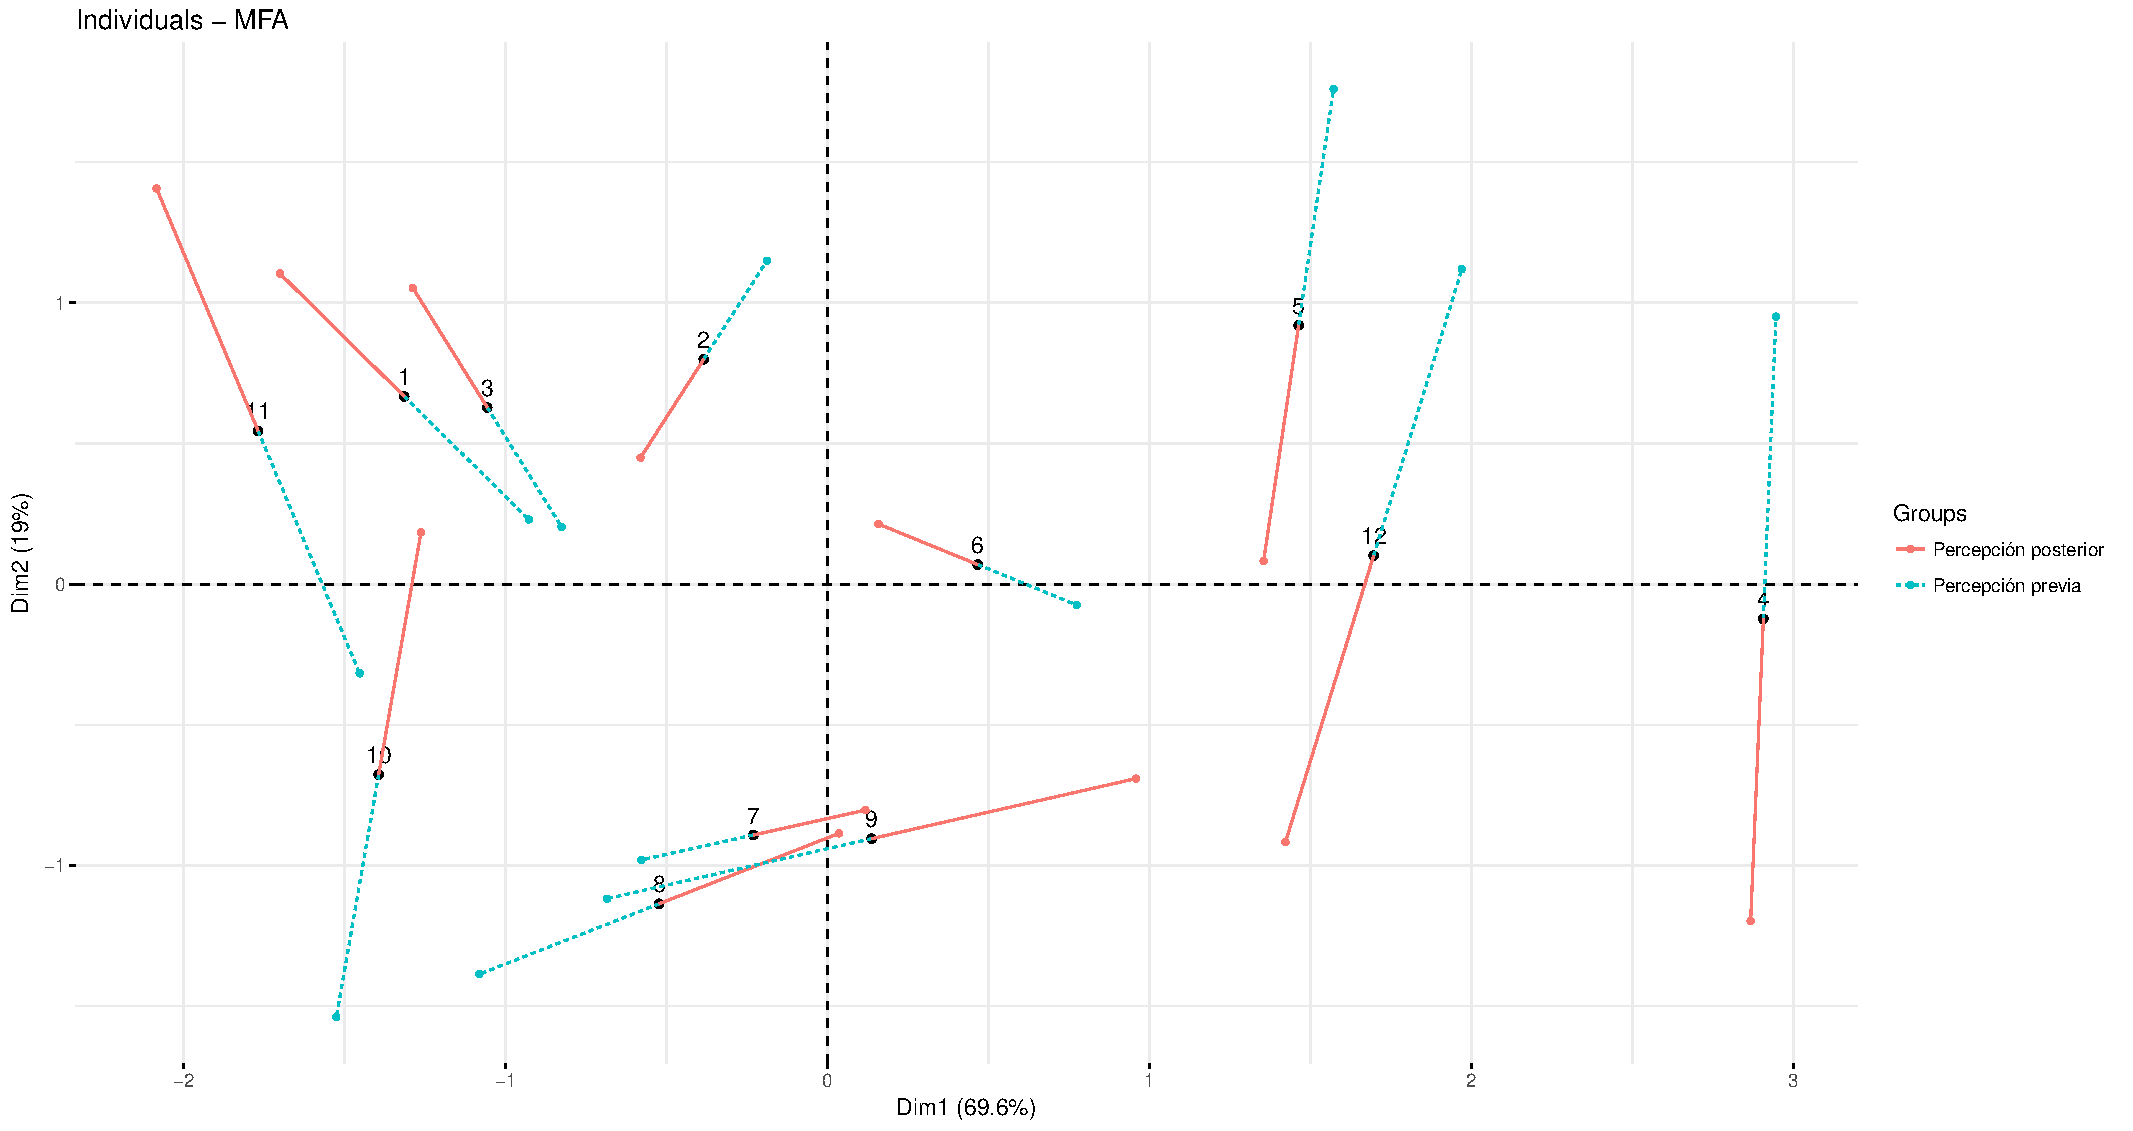
\includegraphics[scale=0.34]{imagenes/RS.pdf}
\end{figure}
\end{frame}

\begin{frame}
\frametitle{Ejes parciales}
\begin{figure}[h]
  \centering
  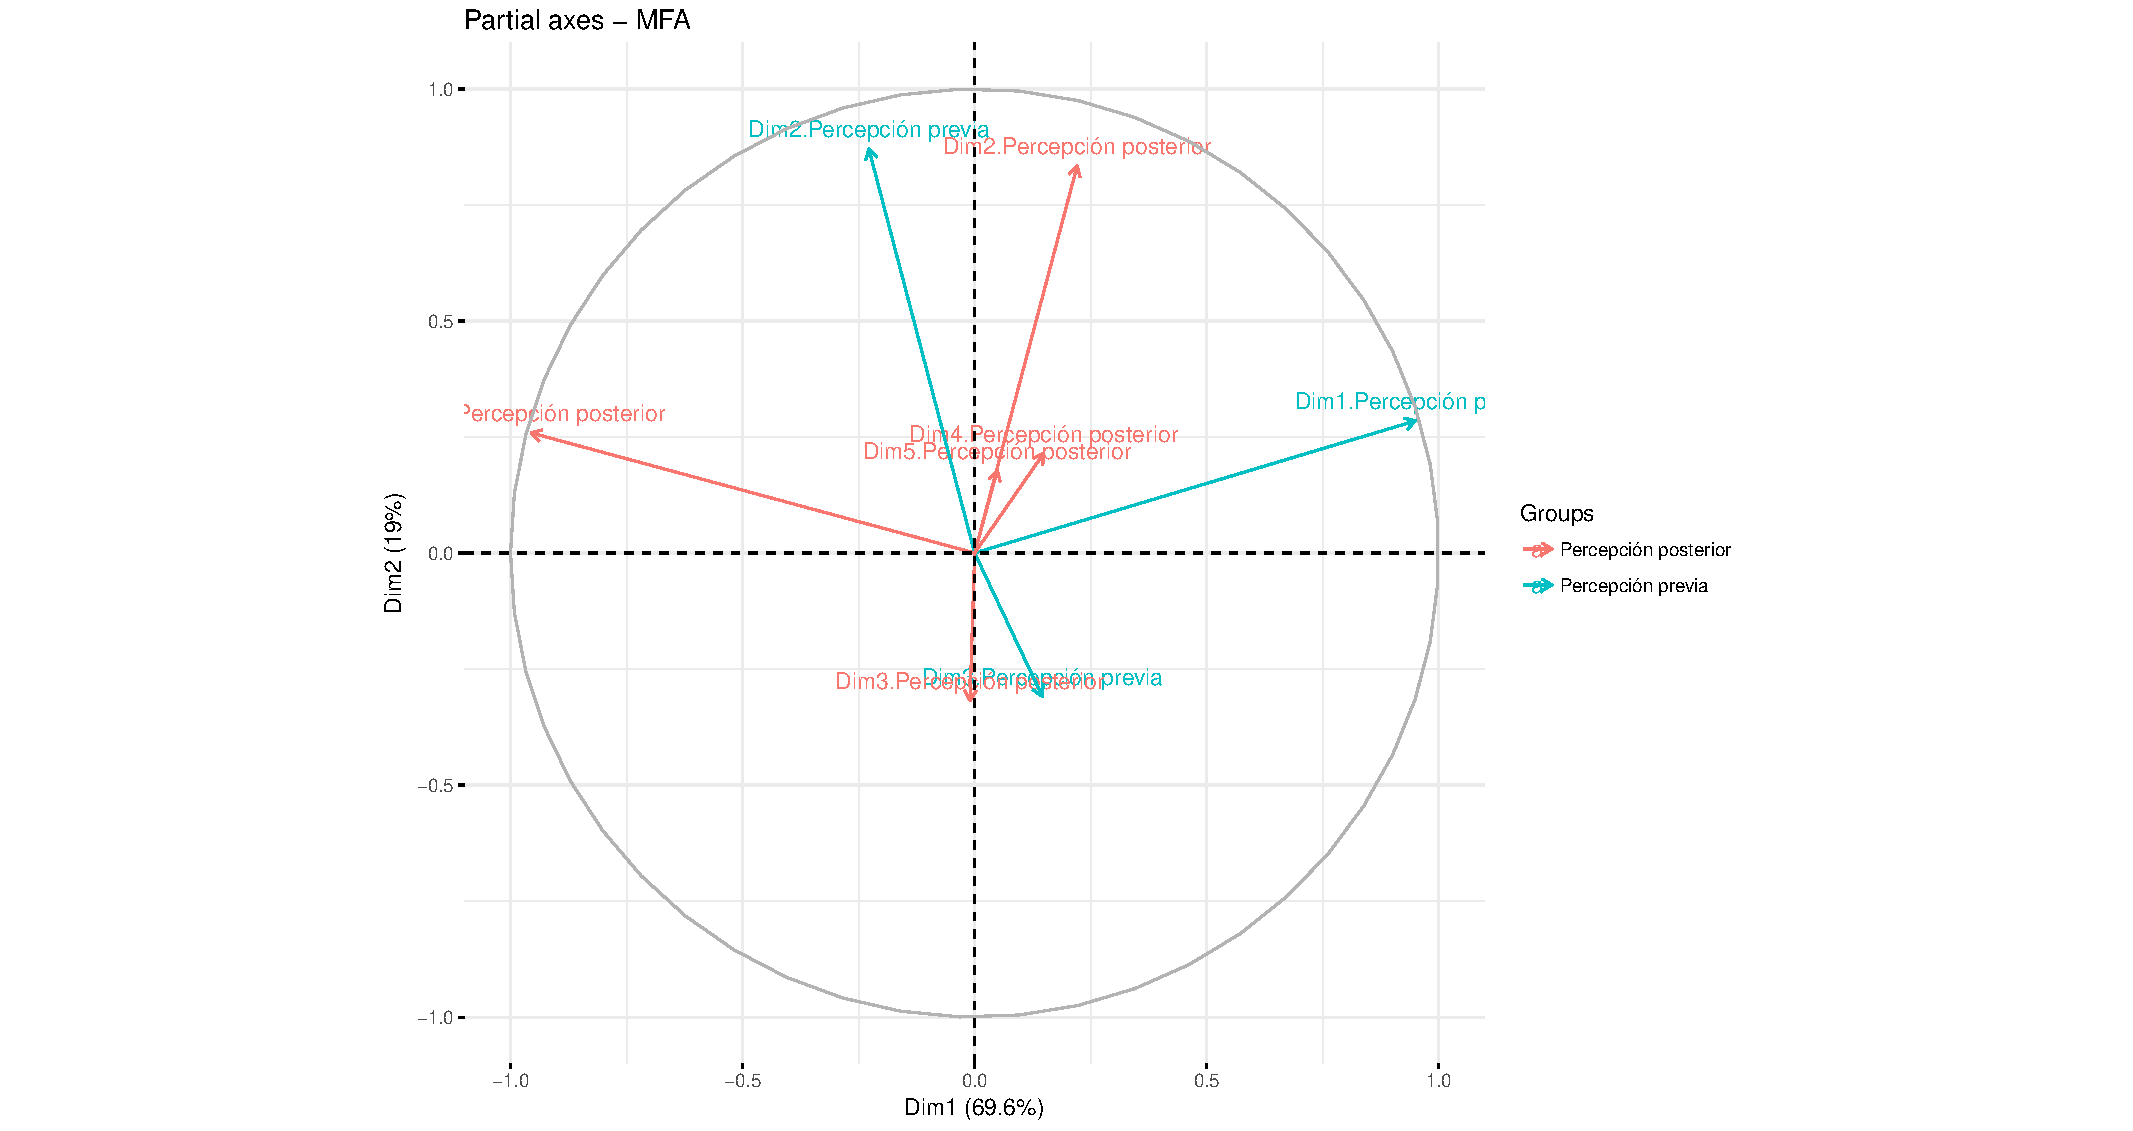
\includegraphics[scale=0.34]{imagenes/EP.pdf}
\end{figure}
\end{frame}

\begin{frame}
\frametitle{Construcción indice}
Las coordenadas de las variables para las dos primeras dimensiones son:

\begin{center}
\resizebox{10cm}{!}{
\begin{tabular}{ccc}
\hline 
 & Dim.1  &    Dim.2   \\   
\hline   
Color.intensity &  0.8581049&  0.2236407 \\ 
Odor.intensity  &  0.6316557&  0.7028833 \\
Attack.intensity & 0.9522195& -0.2260020  \\
Sweet           & -0.8881581& -0.1346408  \\
Acid             & 0.9028145& -0.3139184  \\
Bitter           & 0.9640321&  0.1981328 \\
Pulp             &-0.6320766&  0.7018089 \\
Typicity         &-0.8054955&  0.3978624  \\
\hline
\end{tabular}
}
\end{center}
\end{frame}

\begin{frame}
\frametitle{Construcción indice}
~\\El indice para el primer grupo (percepción previa) es:
$$I=0.8581049 Color+0.6316557 Odor+0.9522195 Attack$$
\begin{center}
\resizebox{3cm}{!}{
\begin{tabular}{cc}
\hline 
 Jugo & Indice  \\   
\hline   
1 & 11.03415 \\
2 &  11.823 \\
3 & 11.16971\\ 
4 & 16.35666\\
5 & 14.28656\\ 
6 & 13.58883\\ 
7 & 11.71434\\ 
8 & 11.12588\\ 
9 & 11.61305\\ 
10& 10.57015\\ 
11& 10.35774\\ 
12& 14.9813 \\  
\hline
\end{tabular}
}
\end{center}
\end{frame}

\begin{frame}
\frametitle{Referencias}
\begin{itemize}
\item Kassambara, A. \& Mundt, F. (2017), factoextra: Extract and Visualize the Results of Multivariate
Data Analyses. R package version 1.0.5.
*https://CRAN.R-project.org/package=factoextra


\item Lê, S., Josse, J. \& Husson, F. (2008), 'FactoMineR: A package for multivariate analysis', Journal
of Statistical Software 25(1), 1-18.


\item Ludovic Lebart, Alain Morineau, M. P. (1995), Statistique exploratoire multidimensionnelle, Dunod,
Paris.

\item Salamanca, J. A. C. (2017), 'Análisis factorial múltiple para clasificación de universidades latinoamericanas', Comunicaciones en Estadística .
\end{itemize}
\end{frame}

\begin{frame}
\frametitle{Referencias}
\begin{itemize}
\item Wickham, H. (2009), ggplot2: Elegant Graphics for Data Analysis, Springer-Verlag New York.
*http://ggplot2.org


\item Wickham, H. \& Bryan, J. (2018), readxl: Read Excel Files. R package version 1.1.0.
*https://CRAN.R-project.org/package=readxl


\item Zelaya, J. T. (n.d.), ANÁLISIS MULTIVARIADO DE DATOS, Universidad de Costa Rica.
\end{itemize}
\end{frame}

\end{document}